\documentclass[12pt]{article}
        \usepackage{graphicx,type1cm,eso-pic,color}
        \usepackage{hyperref}
        \usepackage[left=3.0cm,right=3.0cm,top=2cm,bottom=2cm,headheight=13.6pt]{geometry}
       %\usepackage{subfigure}

\makeatother
\begin{document}

\rightline{October 28 2016}
\rightline{Version V1.0}
\vskip 0.5cm
\begin{center}

\begin{figure}[htbp]
\begin{center}
\vspace{0cm}
%\includegraphics[scale=0.50]{tdr_figs/ft.eps}
\includegraphics[scale=0.5]{pics/ft-drawing.eps}
\end{center}
\end{figure}

\vskip 1.5cm

{\huge\bf\bf CLAS12}
\vskip 0.5cm

{\huge\bf\bf Forward Tagger (FT)}
\vskip 0.5cm


{\huge\bf Manual of operation}
\vskip 0.8cm
{\large\bf The CLAS12 Collaboration}
\vskip 0.5cm
\end{center}

\small
\newpage


\vskip 2.5 cm
\abstract{
This manual describes how to operate the CLAS12-Forward Tagger (FT).The FT is made by three subsystems: an electromagnetic calorimeter (FT-Cal), a hodoscope (FT-Hodo) and a tracker (FT-Trck). This document is divided in three sections, one for each detector.}
\vskip 0.5cm



\newpage

\title{Manual for CLAS12 FT-Cal v1.0} 

%\author{FT-Cal On-Call Cell Phone: 757-810-1489 \\ 
%Authors: \\
%General contact: Marco \textsc{Battaglieri} (\texttt{battagli@jlab.org})\\ 
%LED system: Andrea \textsc{Celentano} (\texttt{andrea.celentano@ge.infn.it})\\
%LV/HV/Chiller/Temps/Scalers: Nathan \textsc{Baltzell} (\texttt{baltzell@jlab.org})\\
%}

%\date{\today} %01/07/2014


\begin{document}
\maketitle{}

\tableofcontents

\newpage
   \section{General description of the FT-Cal}


   The electromagnetic calorimeter (FT-Cal), installed upstream of the CLAS12 torus magnet (Figure~\ref{GView}), is one of the three subsystem of the CLAS12 Forward Tagger and performs two essential functions for the system: it measures the energy of electrons via the detection of the electromagnetic shower and provides input for the trigger system. The FT-Cal modules are based on rectangular 200 mm long PbWO crystal with a 15x15 mm$^2$ face wrapped in VM2000 multilayer polymer mirror film. The scintillation light, approximately 120 photons/MeV at $120^{\circ}$ C and 170 photons/MeV at $0^{\circ}$ C, is read out by a 10x10 mm$^2$ Hamamatsu S8664-1010 Avalanche Photodiode (APD) with 75\% quantum efficiency glued to the rear face surface. The low gain of APDs (150 pC/pC) is compensated with custom-made preamplifier boards, which provide a factor of 600 amplification of the APD signal. In front of the crystals, LEDs are installed to send light into the crystals. These are used in order to check the proper functioning of the FT-Cal and provides complementary information to evaluate gain variations in the various channels of the calorimeter (see Figure~\ref{AmplChain}).

%\%\%\%\%\%\%\%\%\%\%\%\%\%\%\%\%\%\%\%\%\%\%\%\%\%\%\%\
\begin{figure}[htpb]\center
  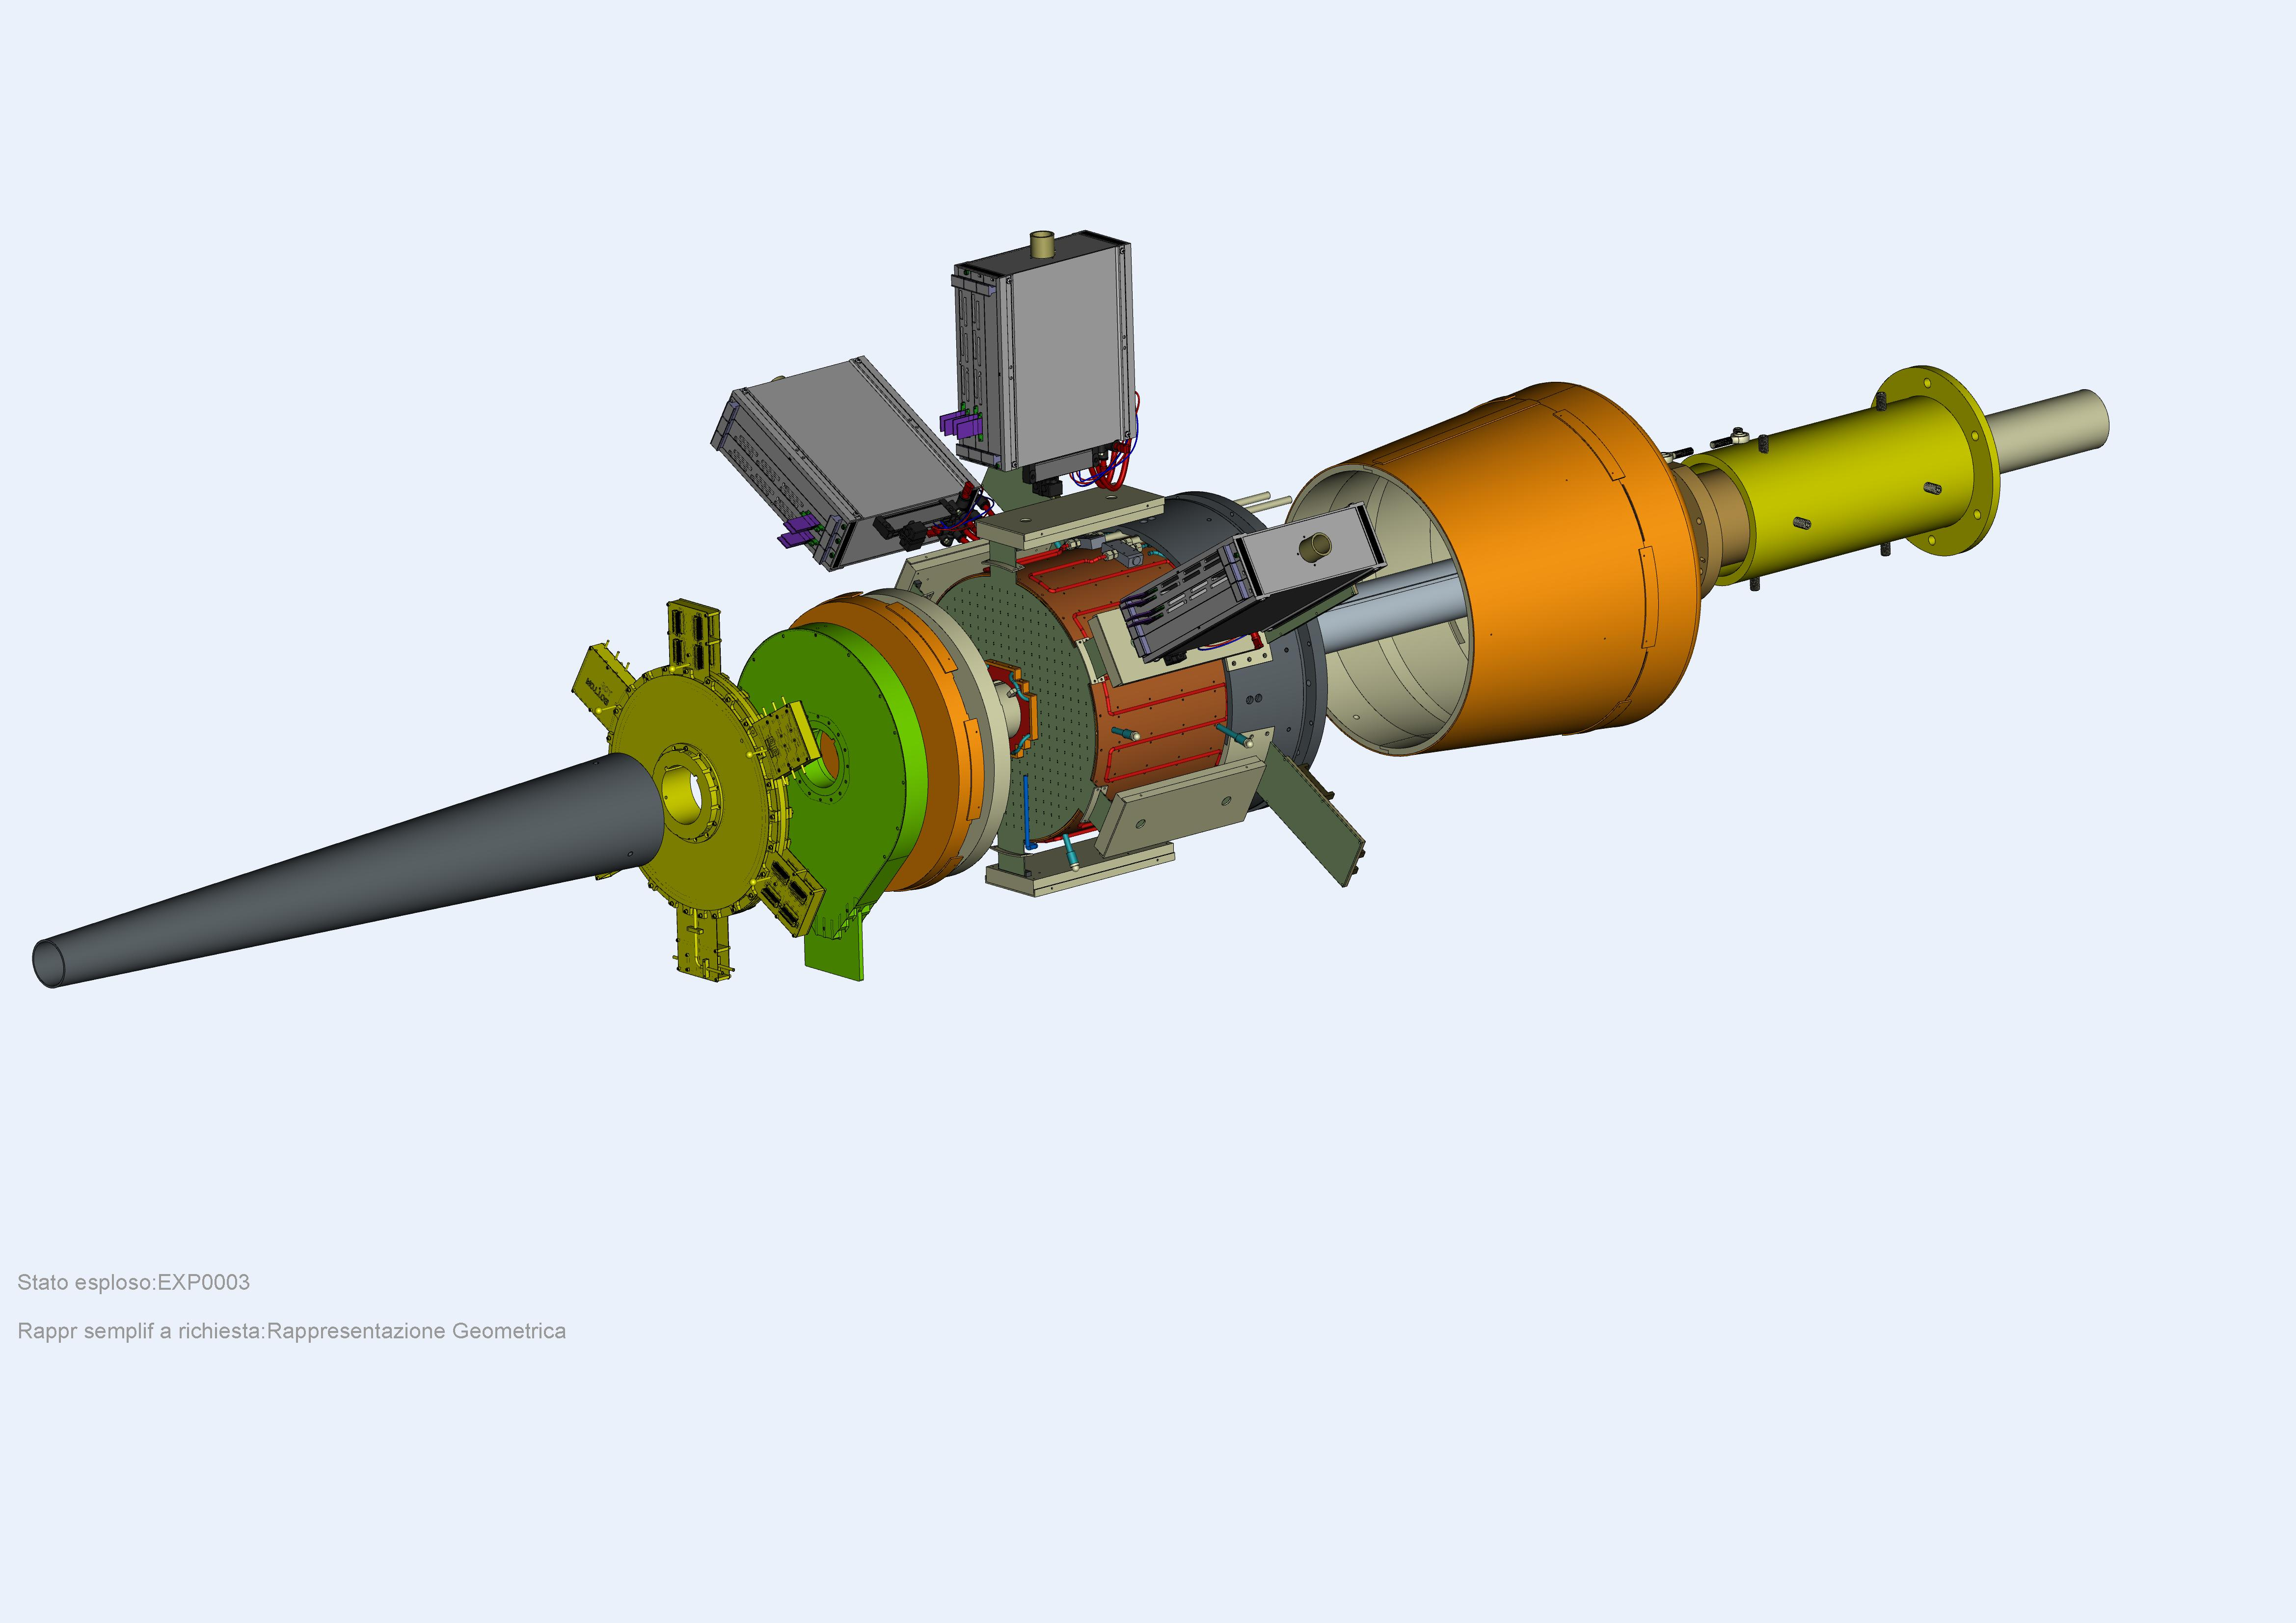
\includegraphics[width=0.75\textwidth]{pics/forward_tagger.jpg} 
  \caption{\label{GView} General view of the Forward Tagger(FT); components shown are the tracker, hodoscope and calorimeter respectively.}
  
\end{figure}
%\%\%\%\%\%\%\%\%\%\%\%\%\%\%\%\%\%\%\%\%\%\%\%\%\%\%\%\      
The FT-Cal is built as a circular matrix of crystals, surrounding the beamline. The 332 modules (Figure~\ref{fig:Crystals}) are enclosed in a copper structure connected to the calorimeter cooling circuit ( $< 1^\circ$C stability and $< 1^\circ$C uniformity) to stabilize the crystal light yield and the operation of the APDs. Two semi-circular printed circuit boards (referred as mother boards) mounted on the back plane with two extensions that exit from the enclosure are used to supply the $\pm5$ V operating voltage for the preamplifiers, the 400 V bias voltage to the APDs, and to read out signals from the APDs. Each half of the FT-Cal is divided into 18 bias voltage groups formed in order to minimize the gain spread of the APD-preamplifier couples.
%\%\%\%\%\%\%\%\%\%\%\%\%\%\%\%\%\%\%\%\%\%\%\%\%\%\%\%\
\begin{figure}[htpb]\center
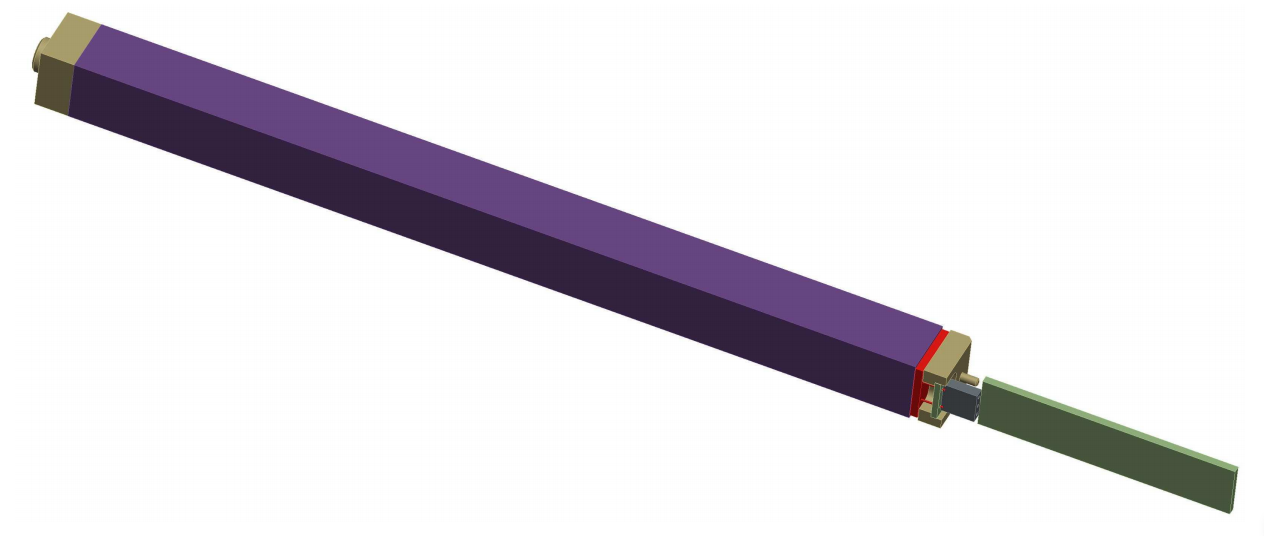
\includegraphics[width=0.75\textwidth]{pics/CrystalAssembly.PNG}
\caption{\label{AmplChain} View of an FT-Cal crystal and the amplification chain.}
\end{figure}
%\%\%\%\%\%\%\%\%\%\%\%\%\%\%\%\%\%\%\%\%\%\%\%\%\%\%\%\
After a 1:1 signal splitter, 1/2 of an amplified APD signal is fed to a single channel of a JLab flash ADC (FADC) board. The FADC boards are high speed VXS modules digitizing up to 16 crystal signals at 250 MHz and storing 4 ns samples with 12-bit resolution. When a trigger is received, the pipeline is read on these boards from 5 samples before and 30 after the trigger time (those values will be adapted during commissioning).


%\%\%\%\%\%\%\%\%\%\%\%\%\%\%\%\%\%\%\%\%\%\%\%\%\%\%\%\
\begin{figure}[htpb]\center
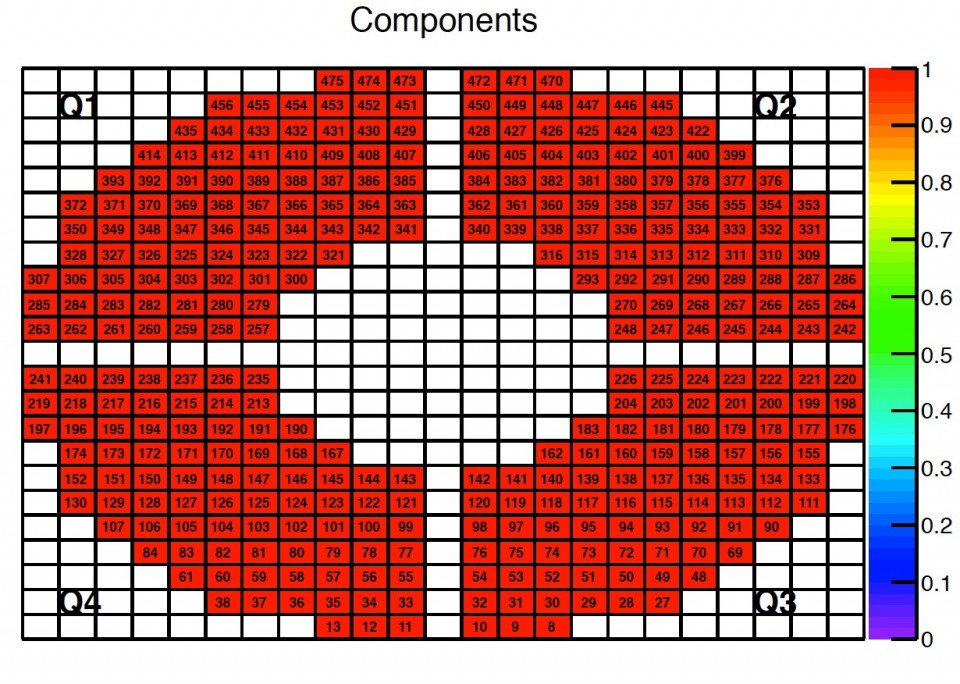
\includegraphics[width=0.75\textwidth]{pics/FT-CalMap-Component.jpg}
\caption{ \label{fig:Crystals} Front view of the FT-Cal crystals layout, with indications of the component number.}
\end{figure}
%\%\%\%\%\%\%\%\%\%\%\%\%\%\%\%\%\%\%\%\%\%\%\%\%\%\%\%\


 \twocolumn
\part{Shift Takers Instructions}

\vspace*{\stretch{1}}      
All FT-Cal controls are accessible through EPICS, from the main CLAS12\_EPICS window (Figure~\ref{fig:EPICSmain}).  If not already running, it can be opened by executing
the command \begin{center}\texttt{clas12\_epics}\end{center} in a terminal on any of
the \texttt{clonpc\#\#} workstations in the Hall-B counting house.

{\em   All shift workers should be using user \texttt{clasrun} for all instructions in this document.}

The primary FT-Cal screen is shown in Figure~\ref{fig:ecal_all} and opened via the standard CLAS EPICS control GUI.
\vspace*{\stretch{1}}      
%\%\%\%\%\%\%\%\%\%\%\%\%\%\%\%\%\%\%\%\%\%\%\%\%\%\%\%\
\begin{figure}[h!]
\center
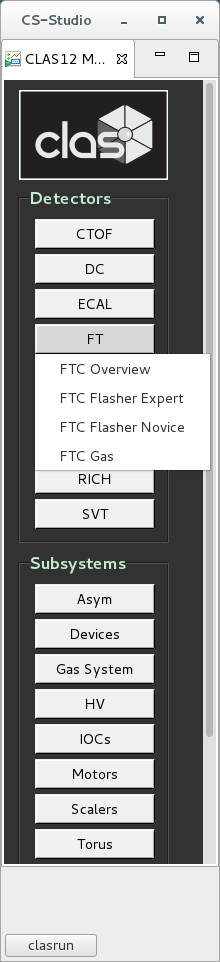
\includegraphics[width=0.30\textwidth]{pics/clascss_main_menu_FT_selection.png}
\caption{ \label{fig:EPICSmain} View of the Hall-B EPICS main window.Menu shown gives access to the HV, LV, Temperature sensors, Chiller, Gas system, and LED flasher.}
\end{figure}
%\%\%\%\%\%\%\%\%\%\%\%\%\%\%\%\%\%\%\%\%\%\%\%\%\%\%\%\
 \onecolumn

 \section{Primary FT-Cal EPICS Screen}\label{sec:ft-epics}
 This one screen combines all basic FT-Cal EPICS controls and monitoring into one window.  It is accessible from the {\bf FT} button in Figure~\ref{fig:EPICSmain}.  This includes embedded versions of the dedicated screens in the following sections:  temperature sensors, chiller, and low and high voltage.  
 
 This screen provides the only FT-Cal {\em controls} shift workers should need, which is to turn LV and HV on and off.  HV should be turned on always after LV. However, this should be supplemented by the strip charts for temperature and HV current, as well as cctv webcams, for additional {\em monitoring} in the following sections.

The grey square buttons in the top right of each section of this main FT-Cal screen provide
access to more detailed or expert screens for the corresponding subsystem.

%\%\%\%\%\%\%\%\%\%\%\%\%\%\%\%\%\%\%\%\%\%\%\%\%\%\%\%\
\begin{figure}[htbp]\centering
    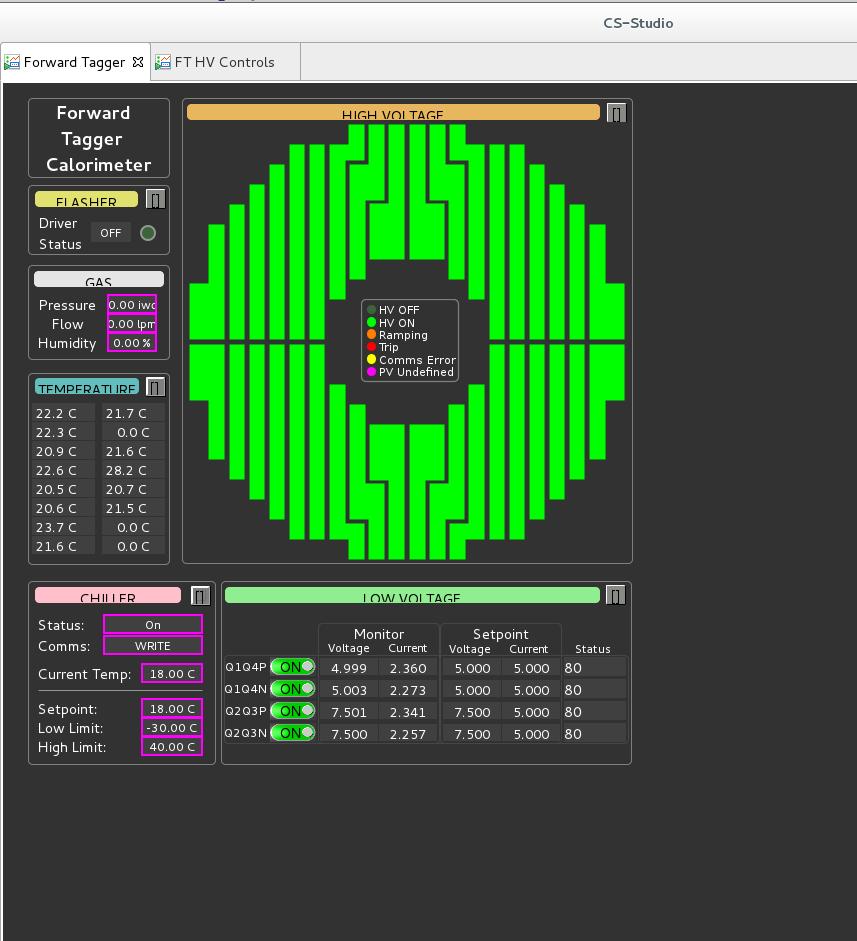
\includegraphics[width=15cm]{pics/All_Working_HVs.png}
    \caption{The primary EPICS screen needed for shift workers to monitor FT-Cal.\label{fig:ecal_all}}
\end{figure}
%\%\%\%\%\%\%\%\%\%\%\%\%\%\%\%\%\%\%\%\%\%\%\%\%\%\%\%\

\newpage
\section{Temperature}\label{sec:ft-t}
The FT-Cal temperature should remain stable within $\pm 0.1^{\circ}$ C   in order to avoid gain variation in the system.  Cooling controls and monitoring are desribed in this section.

\subsection{Temperature Sensors}
Sixteen temperature sensors are placed in the FT-Cal enclosure and should be monitored through FT-Cal's main EPICS screen. Figure \ref{fig:temp} shows the expert screen accessible via the grey square button in the top right of the temperature section of the main FT-Cal screen. Temperatures at different locations in the calorimeter as shown in Figure \ref{fig:temp1} are measured by the instruments shown in Figure~\ref{fig:temp_instruments}. Variations of one degree C or more during a shift should be reported to FT-Cal expert on call and noted in the log book.  The strip charts~\ref{fig:striptemp} are accessible from the two buttons in the temperature section of Figure ~\ref{fig:ecal_all} (and also the main CLAS12\_EPICS screen in Figure \ref{fig:EPICSmain})\footnote{To be implemented.}.


%\%\%\%\%\%\%\%\%\%\%\%\%\%\%\%\%\%\%\%\%\%\%\%\%\%\%\%\
\begin{figure}[htbp]
\center
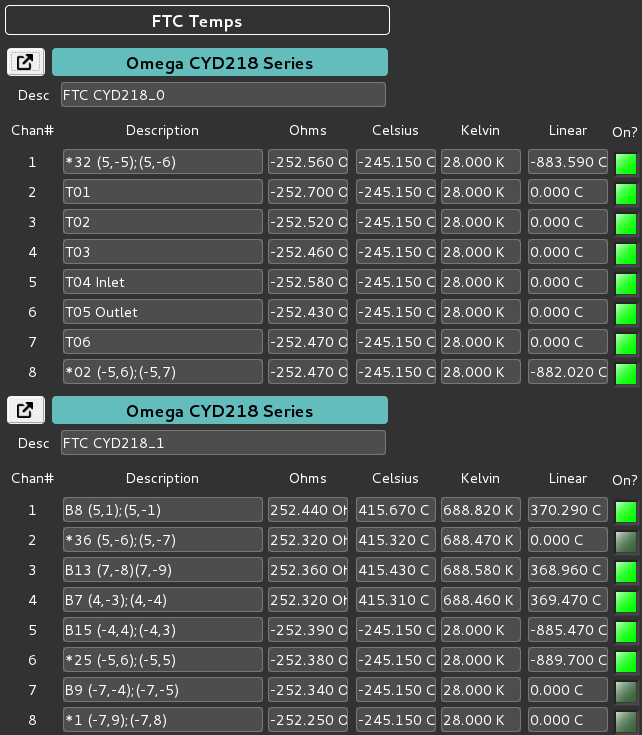
\includegraphics[width=0.75\textwidth]{pics/PT100_3.png}
\caption{ \label{fig:temp} View of the EPICS temperature monitoring window.}
\end{figure}

\begin{figure}[htbp]
\center
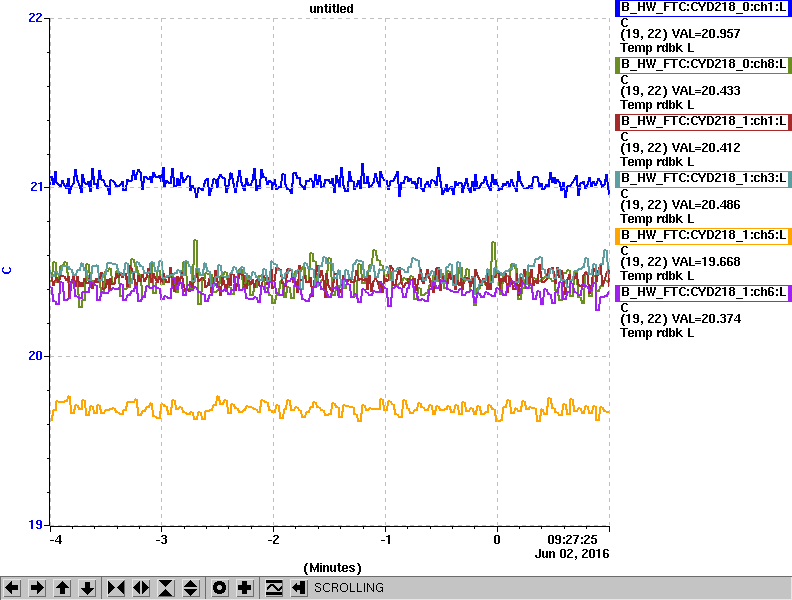
\includegraphics[width=0.75\textwidth]{pics/Strip_Chart_T_Crystal.png}
\caption{ \label{fig:striptemp} Example view of what the implemented EPICS strip charts will look like}
\end{figure}

\begin{figure}[htbp]
\center
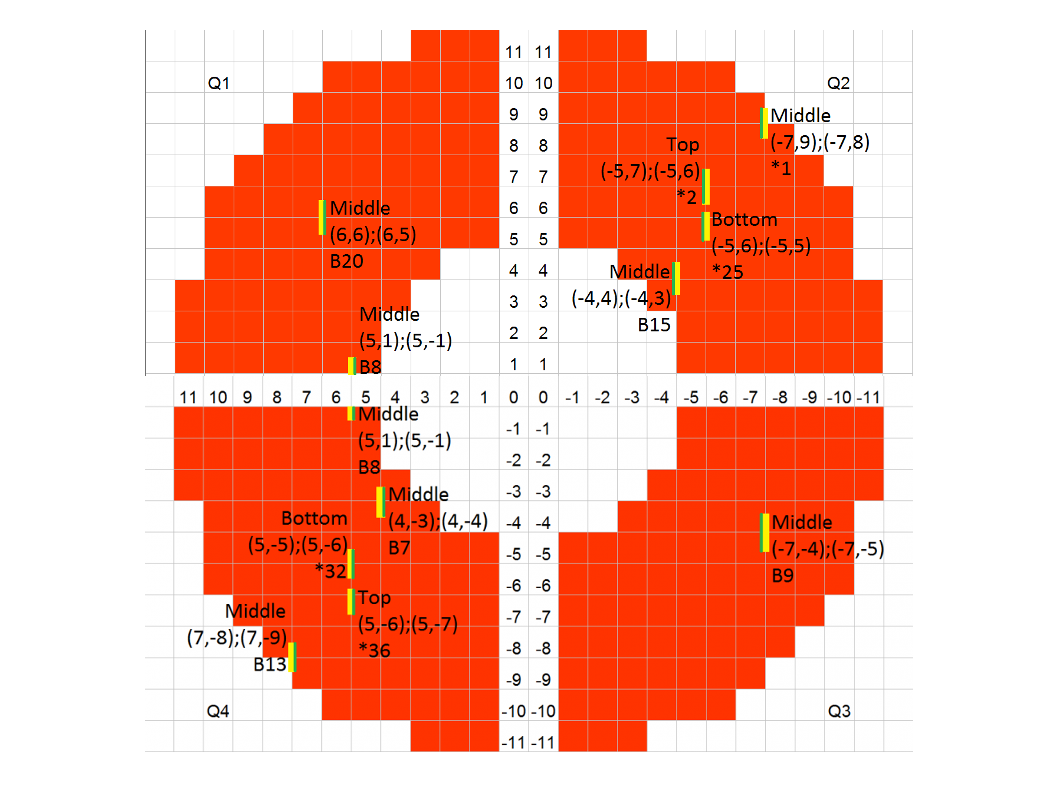
\includegraphics[width=0.75\textwidth]{pics/PT100_crystal_region.png}
\caption{ \label{fig:temp1} Placement of the Flex PT100's within the FTCal.}
\end{figure}
%\%\%\%\%\%\%\%\%\%\%\%\%\%\%\%\%\%\%\%\%\%\%\%\%\%\%\%\
%\
%\\begin{figure}[htbp]
%\\center
%\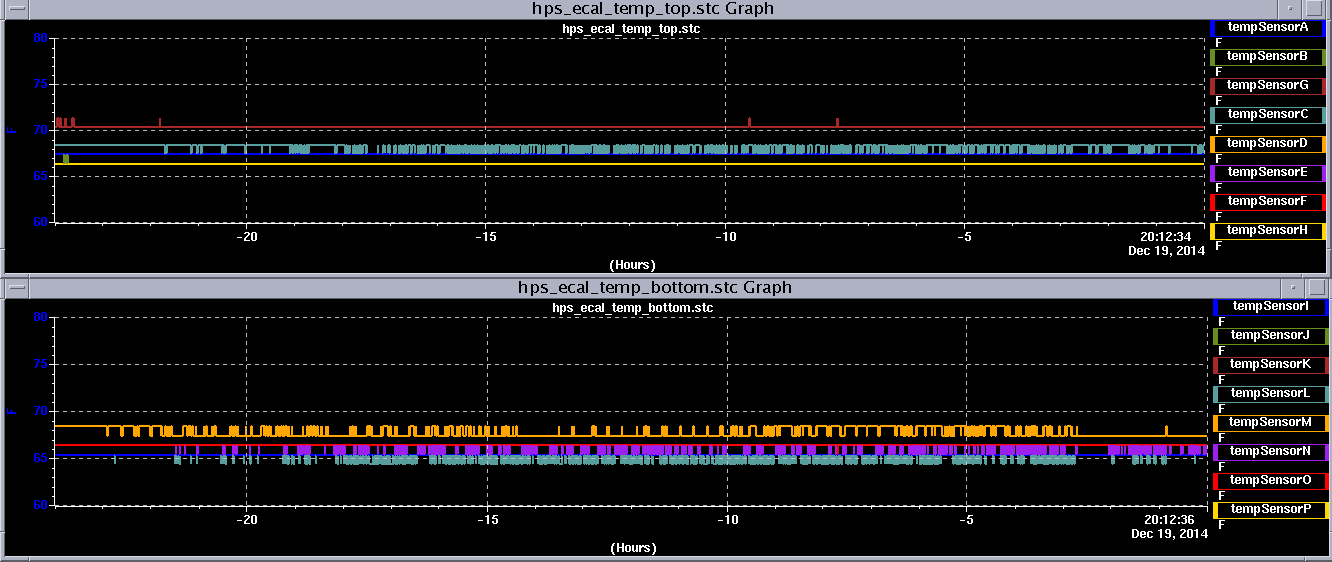
\includegraphics[width=0.45\textwidth,height=4.5cm]{pics/ECal_temp_s.png}
%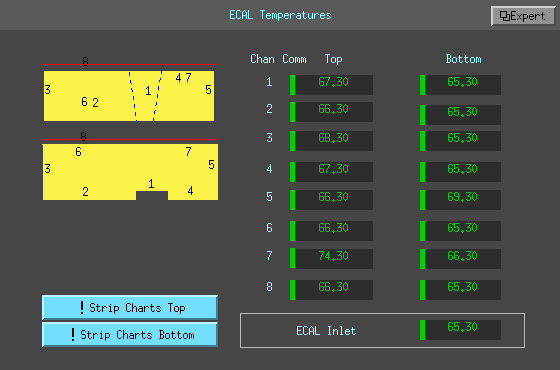
\includegraphics[width=0.39\textwidth]{pics/EcalTemp_2014_12_20.png}
%\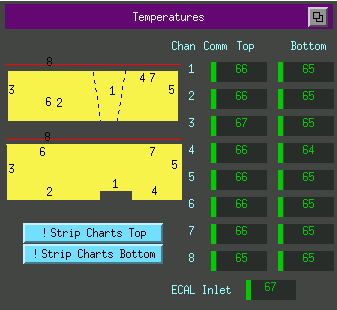
\includegraphics[width=0.3\textwidth,height=4.5cm]{pics/epics_ecal_temp.png}
%\\caption{\label{temp2} View of the EPICS temperature monitoring strip charts (left) and the temperature portion of the main FT-Cal EPICS screen (right).}
%\\end{figure}
%\%\%\%\%\%\%\%\%\%\%\%\%\%\%\%\%\%\%\%\%\%\%\%\%\%\%\%\
%\%\%\%\%\%\%\%\%\%\%\%\%\%\%\%\%\%\%\%\%\%\%\%\%\%\%\%\
\begin{figure}[htbp]
\center
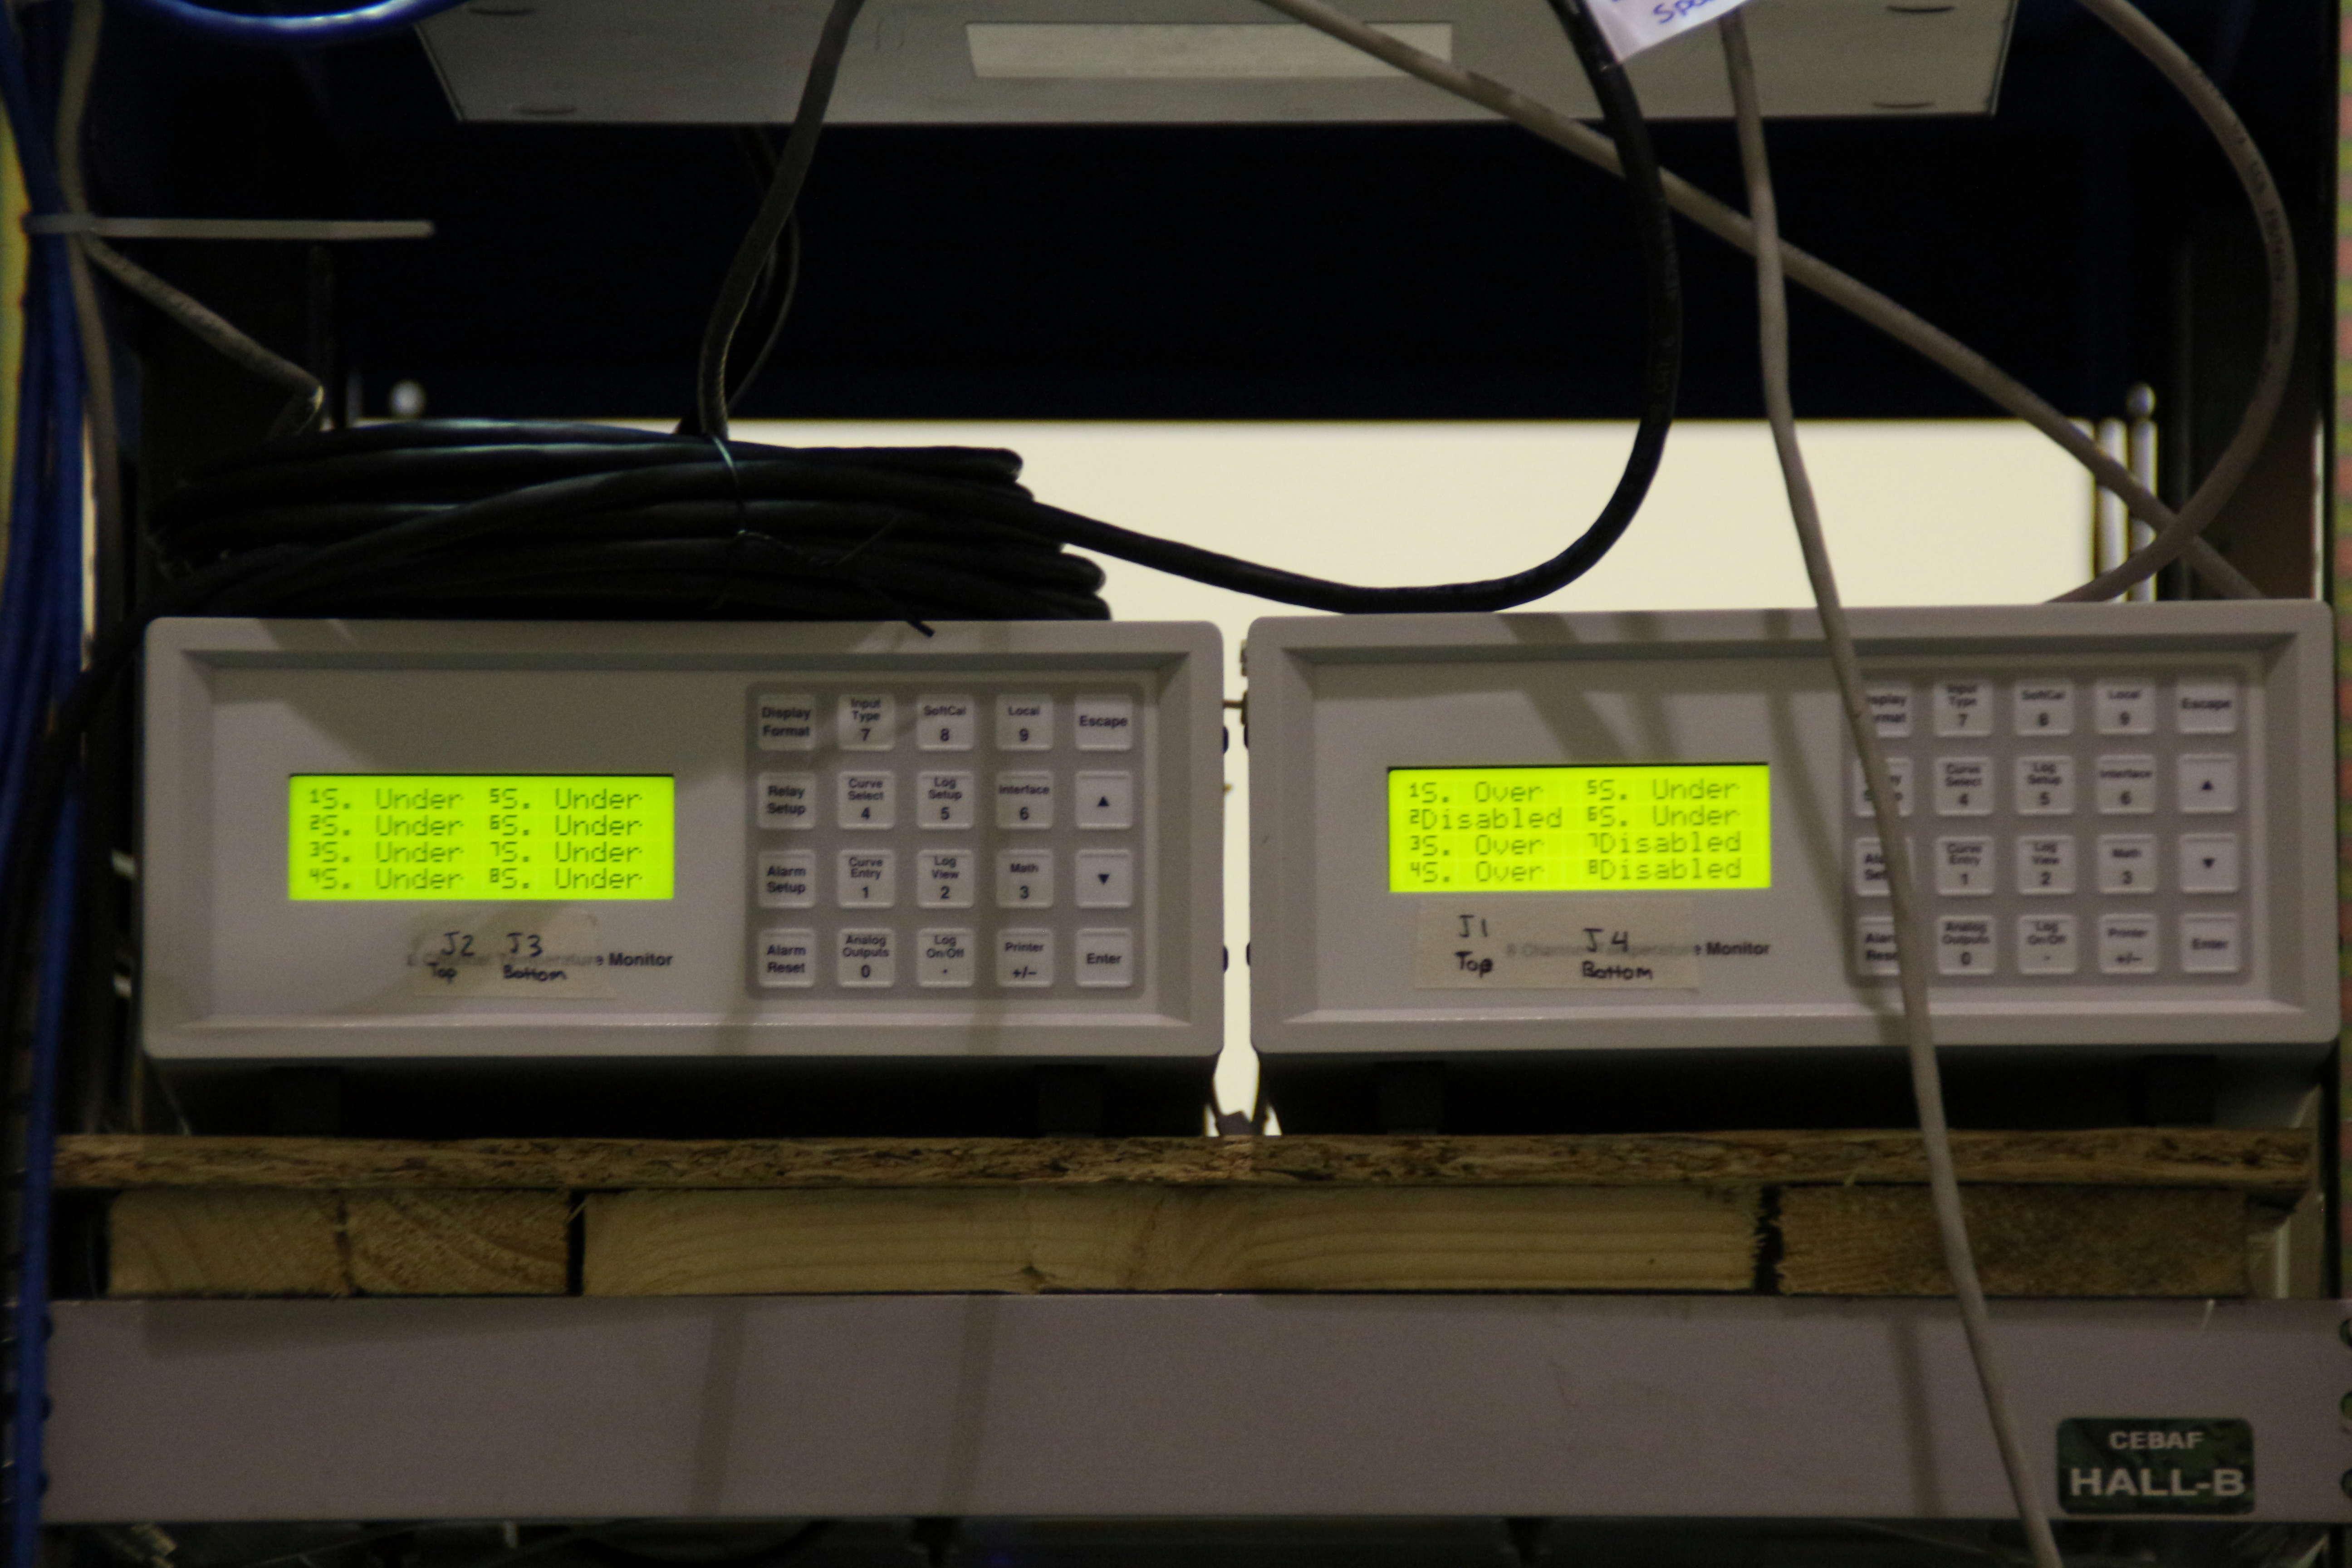
\includegraphics[width=0.45\textwidth,height=4.5cm]{pics/OMEGA.jpg}
\caption{\label{fig:temp_instruments} View of the temperature modules measuring both the crystal and external temperatures of the FTCal.}
\end{figure}
%\%\%\%\%\%\%\%\%\%\%\%\%\%\%\%\%\%\%\%\%\%\%\%\%\%\%\%\
\subsection{Chiller}\label{sec:ft-chiller}
         The chiller allows to keep the calorimeter at the right temperature and should be ON and set at -3 C at all times. The chiller can be monitored through its webcam and EPICS controls (Figure~\ref{ChillerCam}). Shift takers should not attempt to change the chiller settings and call FT-Cal expert in case of problem. % The webcam is accessible in a web browser via the url \texttt{cctv10.jlab.org} and the ``Monitoring'' tab on the {\bf HPS Run Wiki}.


\begin{figure}[htbp]
\center
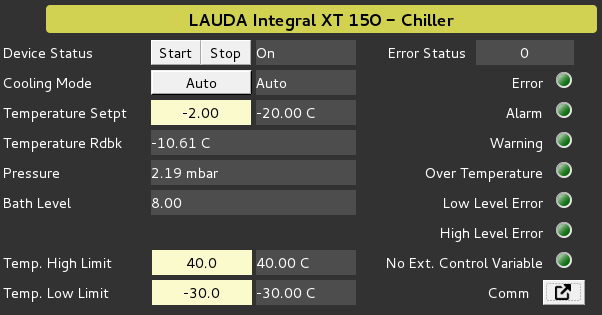
\includegraphics[width=0.99\textwidth]{pics/Chiller_Slwcntrl.png}
\caption{ \label{ChillerCam} View of the chiller slow control window, for the purpose of live monitoring.}
\end{figure}
%\%\%\%\%\%\%\%\%\%\%\%\%\%\%\%\%\%\%\%\%\%\%\%\%\%\%\%\

\newpage

\section{Low Voltage}\label{sec:ft-lv}
{\em The low voltage power supply must be on before HV is turned on, and changing its settings requires contact with an FT-Cal-expert.}
      
LV should be monitored using its portion of the main FT-Cal EPICS screen (shown in Figure~\ref{fig:ecal_all}). The currents driven by the four channels should be similar. Call the FT-Cal expert if this appears not to be ON or shows an abnormal current for any of the channels.  {\em Normal current is between 2.2 and 2.4 A for all channels}. % This webcam is accessible via the url \texttt{cctv11.jlab.org} in a web browser and the ``Monitoring'' tab on the main {\bf HPS Run Wiki}.

%\%\%\%\%\%\%\%\%\%\%\%\%\%\%\%\%\%\%\%\%\%\%\%\%\%\%\%\
\begin{figure}[htbp]
\center
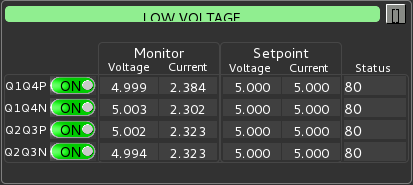
\includegraphics[width=0.5\textwidth,height=5.5cm]{pics/LV.png}
\caption{ LV controls for the FTCal. }
\end{figure}
%\%\%\%\%\%\%\%\%\%\%\%\%\%\%\%\%\%\%\%\%\%\%\%\%\%\%\%\

\section{High Voltage}\label{sec:ft-hv}
      \subsection{Turning ON/OFF High Voltages}

      The high voltage supply of the FT-Cal is controlled and monitored using the main FT-Cal
EPICS window (Figure ~\ref{fig:ecal_all}).  It has buttons to ramp up and down the entire 
calorimeter's high voltages, accessible via the gray square buttom on the top right of the HV section of the main GUI, open windows for
individual channel control (Figure~\ref{fig:HVControl}), and open more detailed expert views.
%(e.g. Figure ~\ref{HV}).

   \subsection{HV Current Monitoring}
   Individual channels' currents can be monitored from the GUI in Figure~\ref{fig:HVControl}, and strip charts should be open for long term monitoring (see Fig. ~\ref{fig:hvcurrentstrips}). % The strip charts are accessible from the main FT-Cal screen (Figure ~\ref{fig:ecal_all}) under the HV sections' {\bf Monitors} button (and also from the HPS\_EPICS screen (Figure~\ref{EPICSmain}) via the {\bf Strip-Tool} button).  An example is shown in Figure~\ref{fig:hvcurrentstrips}. 
 Jumps or drifts in current of more than 1 A should be noted in the logbook.
   
   
%\%\%\%\%\%\%\%\%\%\%\%\%\%\%\%\%\%\%\%\%\%\%\%\%\%\%\%\
  \begin{figure}[htbp]\centering
       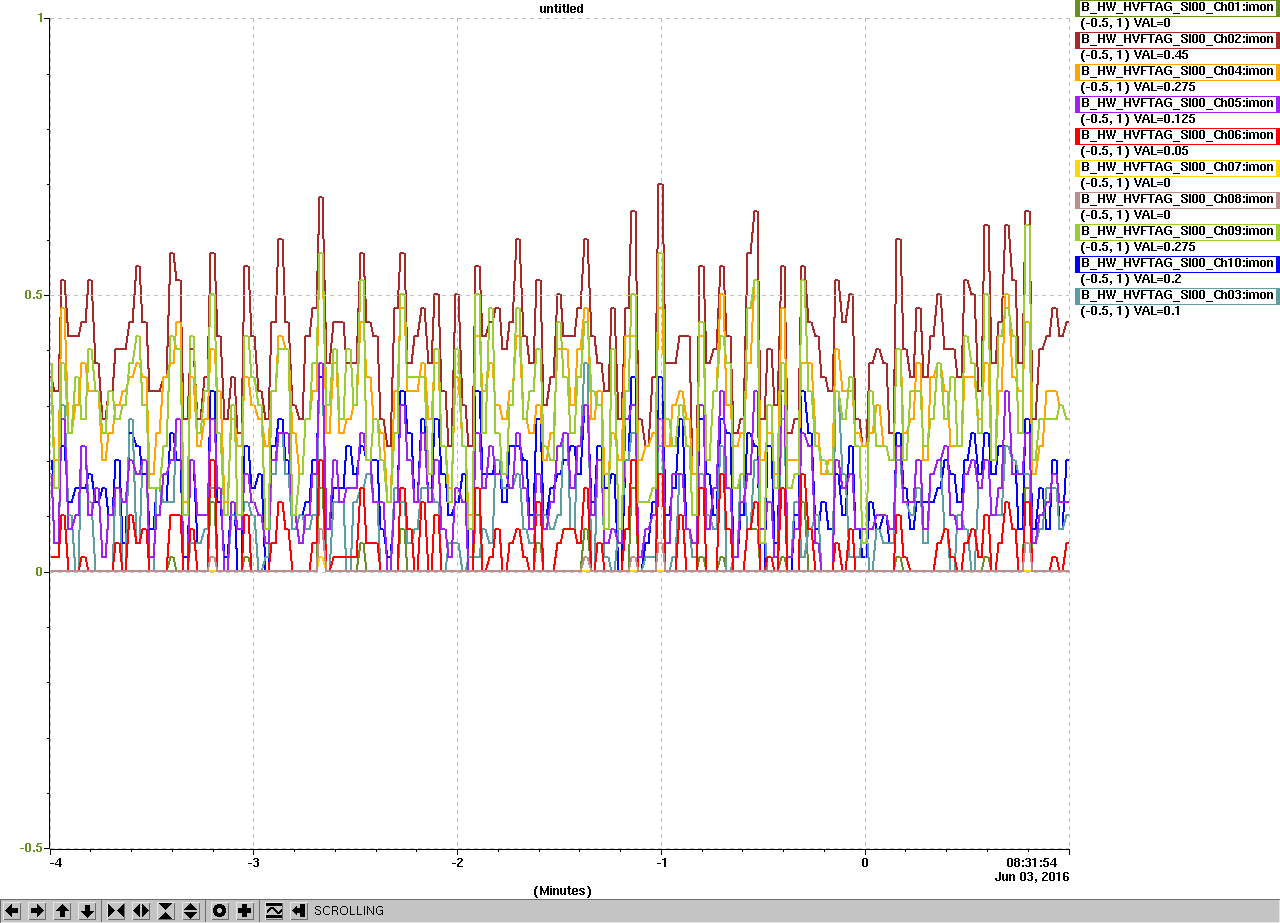
\includegraphics[width=16cm]{pics/HV_I_Strip_Chart.png}
       \caption{Example HV Current strip chart. This feature will be added soon to the FTCal Epics Gui.\label{fig:hvcurrentstrips}}
  \end{figure}
%\%\%\%\%\%\%\%\%\%\%\%\%\%\%\%\%\%\%\%\%\%\%\%\%\%\%\%\

   \subsection{Responding to HV trips}

   HV problems, in particular trips, are indicated by a red group in the main FT-Cal EPICS GUI (Figure~\ref{fig:ecal_all}).  HV trips will also be announced by the alarm handler.  During normal operations with HV ON, there should be no red groups in Figure \ref{fig:ecal_all} and no ECAL HV alarms.  In case of an HV trip, or a red region in Figure \ref{fig:ecal_all}:
\begin{itemize}
    \item Try to reenable the tripped HV group by turning it back on in the EPICS HV control screen (Figure~\ref{fig:HVControl}) accessed via the {\bf Controls} button in the menu accessiable via the gray square button of the HV section the main FT-Cal EPICS screen (Figure \ref{fig:ecal_all}). 
% (An easier alternative is just pressing the {\bf ALL ON} button in the main FT-Cal EPICS screen.)
    \item Record the trip in the log book with precise indication of the group and run
        number concerned. 
\end{itemize}
Contact the ECAL expert on-call in case of uncertainty.
      
      {\em Note, the HV can take up to 1 minute to turn back on so you should end the current run and begin a new one when the high voltage is back on. If you cannot get a HV group to work contact the FT-Cal expert on call.}

      {\bf If you encounter more than two HV trips during your shift for the same group, you should notify the FT-Cal Expert.}


%\%\%\%\%\%\%\%\%\%\%\%\%\%\%\%\%\%\%\%\%\%\%\%\%\%\%\%\
\begin{figure}[htbp]
\center
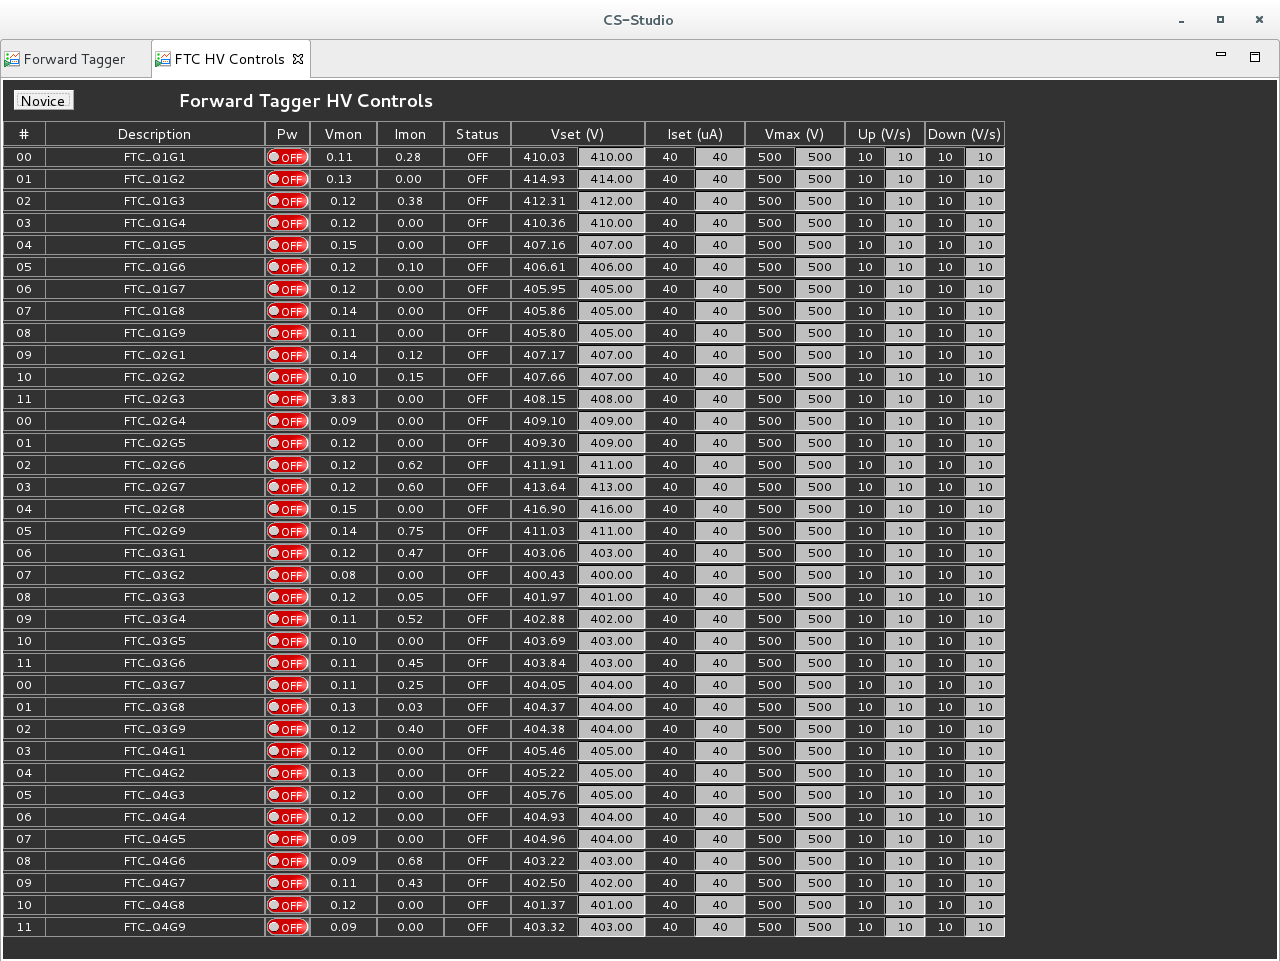
\includegraphics[width=0.85\textwidth]{pics/FTC_HV_controls_expert.png}
\caption{ \label{fig:HVControl} View of the EPICS FT-Cal HV control window for individual channels.}
\end{figure}
%\%\%\%\%\%\%\%\%\%\%\%\%\%\%\%\%\%\%\%\%\%\%\%\%\%\%\%\

 \section{How to switch ON/OFF the FT-Cal}
As discussed in the previous Secs. the FT-Cal to operate requires to have the LV, HV and the chiller on. Here below is the sequence of operations required.
\subsection{Switching the FT-Cal ON}
\begin{itemize}
\item{From  the CLAS12 EPICS control   bring the Primary FT-Cal EPICS screen ON (see Sec.\ref{sec:ft-epics} )}
\item{Check temperatures (see Sec.\ref{sec:ft-t}) and the status of the chiller (see Sec.\ref{sec:ft-chiller}), if OFF, do not proceed and  call the FT-Cal expert.}
\item{Switch the LV ON (see Sec.\ref{sec:ft-lv})}
\item{Switch the HV ON (see Sec.\ref{sec:ft-hv}) {\it HV has to  be switched ON AFTER LV!}}
\end{itemize}

\subsection{Switching the FT-Cal OFF}
\begin{itemize}
\item{From  the CLAS12 EPICS control   bring the Primary FT-Cal EPICS screen ON (see Sec.\ref{sec:ft-epics} )}
\item{Switch the HV OFF (see Sec.\ref{sec:ft-hv}) {\it HV has to  be switched OFF BEFORE LV!}}
\item{Switch the LV OFF (see Sec.\ref{sec:ft-lv}).}
\item{Leave the chiller ON (see Sec.\ref{sec:ft-chiller})}
\end{itemize}



\clearpage
\newpage
      \section{Scalers}      
Rates seen by the FT-Cal are available in the ROOT-based GUI shown in Figure \ref{Scalers}, which represent the rates as seen by the FADC electronics.This display is currently not accessible via the main clascss window, however it will be implemented in the final version. The current Scaler Gui is stored on the jlab12daq1 machnine located in the EEL, and has been used for the purpose of channel debugging. These numbers should all remain constant within $^\sim10\%$ during stable beam operation. A color code will help the operator to check the scaler uniformity. A strong increase is the indication of bad beam conditions or the presence of a new source of noise in the FT-Cal system.  If the latter case, please contact FT-Cal expert on call.

%\%\%\%\%\%\%\%\%\%\%\%\%\%\%\%\%\%\%\%\%\%\%\%\%\%\%\%\      
\begin{figure}[htbp]
\center
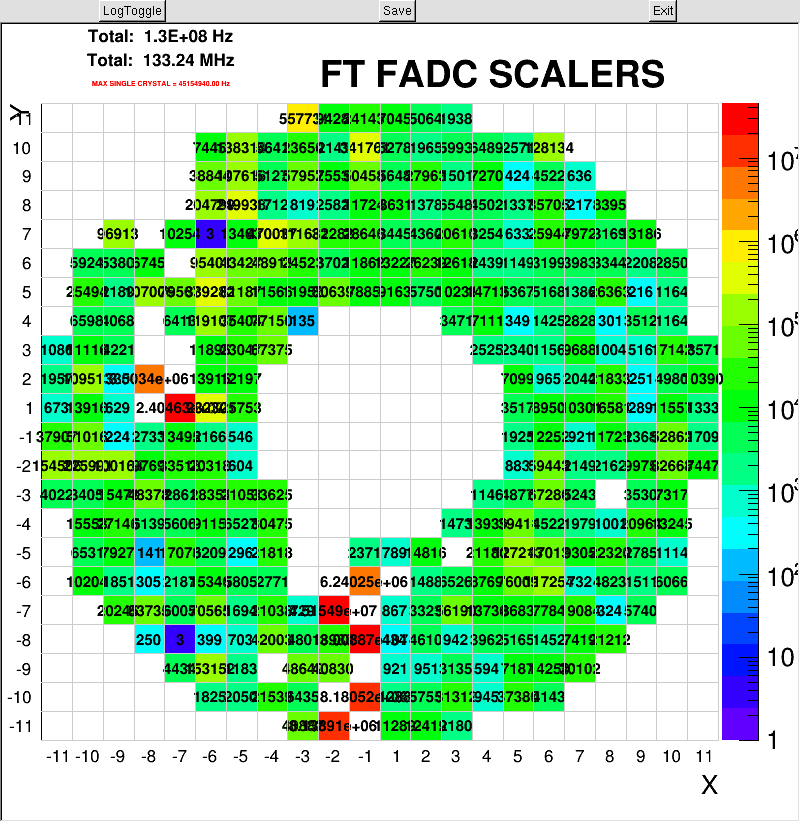
\includegraphics[width=0.8\textwidth]{pics/Scalers.png}
\caption{ \label{Scalers} View of the EPICS FADC scalers window (to be updated based on beam-commissioning rates.}
\end{figure}
%\%\%\%\%\%\%\%\%\%\%\%\%\%\%\%\%\%\%\%\%\%\%\%\%\%\%\%\

\newpage
  \section{Strip Charts}
      The most import quantities to monitor with strip charts are temperature and HV current.  
%There are two programs to view strip charts of FT-Cal EPICS variables.  The older StripTool shown in Figure~\ref{fig:striptemp} can be started from a terminal typing \texttt{StripTool}.  The newer MyaViewer (which adds the ability to retrieve archive information) can be run by executing the following scripts in a terminal (To Be Implemented):
The StripTool from MyaViewer shown in Figure~\ref{fig:striptemp}run by executing the following scripts in a terminal (To Be Implemented):
      
      \begin{itemize}
          \item \texttt{mya\_ftcal\_all.sh}
          \item \texttt{mya\_ftcal\_temp.sh}
          \item \texttt{mya\_ftcal\_curr.sh}
          \item \texttt{mya\_ftcal\_voltage.sh}
      \end{itemize}

\section{Monitoring App}
The CLAS12 java monitoring app is used to run full calorimeter reconstruction and calibration on-line events from the daq on the ET ring.  It provides many plots to assess detector performance.  To start the monitoring app, in a terminal run:
\begin{center}\texttt{clas12-module}\end{center}
and choose from the menu the monitoring application you are interested in.
Then click the ``Et'' button to connect to the ET ring and the ``$>>$'' to start the event processing.

At the start of every run, the histograms in the monitoring app should be cleared via the ``Clear Histograms'' button.  After a few minutes of beam, the tabs should be cycled through and their plots compared to the reference.  Once sufficient statistics are accumulated, snapshot of the relevant panel should be taken and uploaded to the logbook.

\newpage

   \section{LED Monitoring}
      \subsection{System operations}
      The LED system is operated through an EPICS GUI accessible from the main CLAS12 EPICS menu, through FT, then FTC-Flasher Novice (see Figure \ref{FlasherMEDM}).

Shift takers are requested to operate the system in ``Sequence mode'' only. To do so, when requested, click on ``Initialize Flasher'', then verify the TOP frequency is 8000 Hz, and if necessary adjust it trough the proper drop-down menu. Finally, to start the sequence, click on ``Start''. During such a run the DSC scaler screen and the monitoring app allows to check the proper functioning of the channels.% (Figure~\ref{LEDScalers}). 
%\%\%\%\%\%\%\%\%\%\%\%\%\%\%\%\%\%\%\%\%\%\%\%\%\%\%\%\
\begin{figure}[htbp]
\center
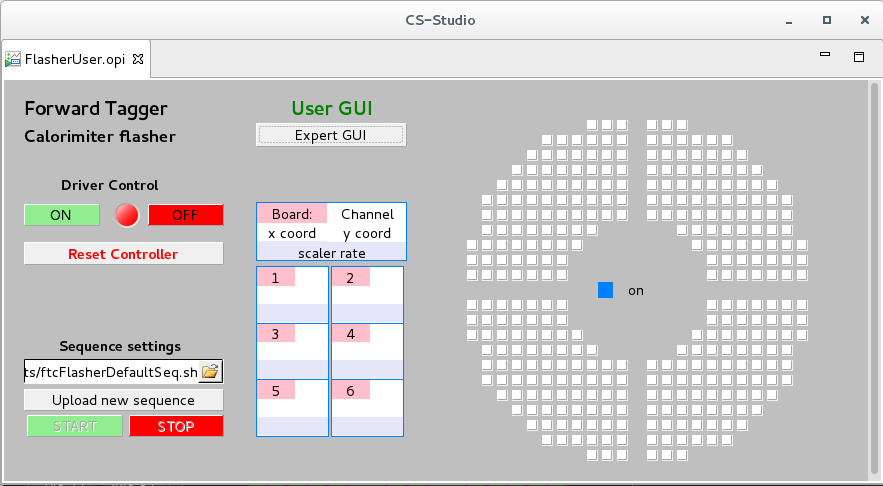
\includegraphics[width=0.75\textwidth]{pics/FTC_flasher.png}
\caption{ \label{FlasherMEDM} The HPS-ECAL Led monitoring system EPICS GUI.}
\end{figure}
%\%\%\%\%\%\%\%\%\%\%\%\%\%\%\%\%\%\%\%\%\%\%\%\%\%\%\%\
%\%\%\%\%\%\%\%\%\%\%\%\%\%\%\%\%\%\%\%\%\%\%\%\%\%\%\%\
%\\begin{figure}[htbp]
%\\center
%\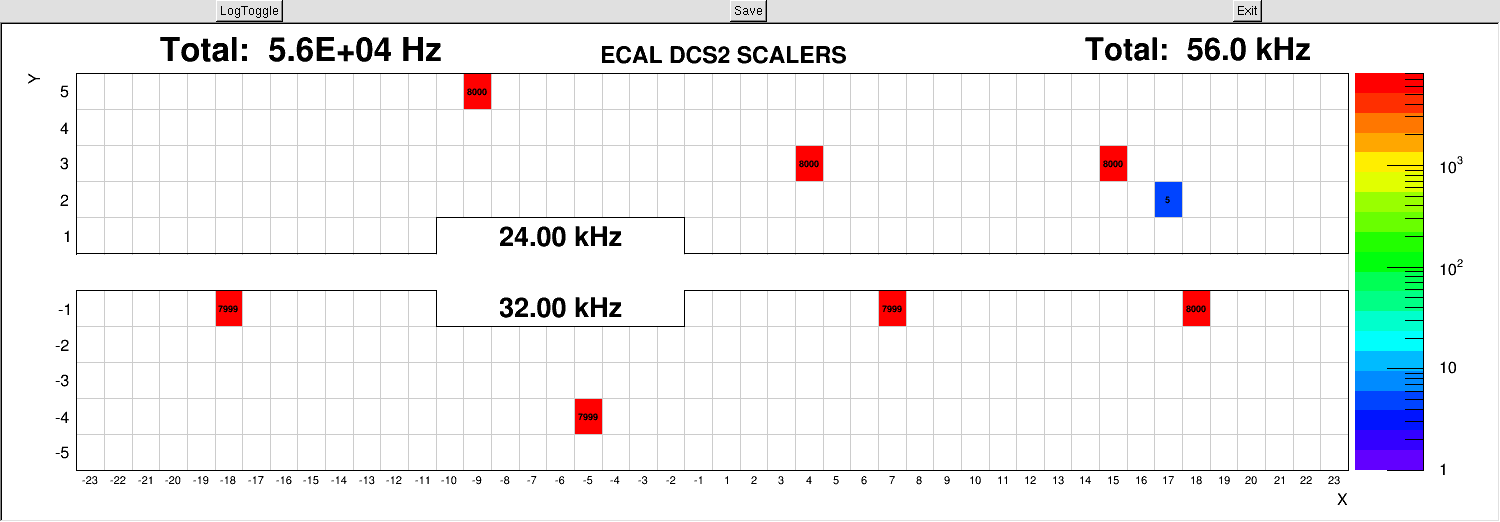
\includegraphics[width=0.95\textwidth]{pics/DSCScalersLED_2014_12_20.png}
%\\caption{ \label{LEDScalers} The HPS DSC scaler during a LED run.}
%\\end{figure}
%\%\%\%\%\%\%\%\%\%\%\%\%\%\%\%\%\%\%\%\%\%\%\%\%\%\%\%\

\subsection{Automatic LED Monitoring}
A monitoring app is setup to record all channels successfully registered during an LED run.  It should be started before the LED sequence is started and viewed afterwards, with the command: \begin{center}\texttt{clas12-module}\end{center} and selecting the FTCalLEDViewerModule from the menu. Make sure to use the clasrun account before using this command.
  
\subsection{Taking a LED sequence run}
The following instructions must be followed to take an LED sequence run. This involves setting the DAQ, starting the LED sequence run, and configure the  monitoring app to monitor the data. At the end of the run, the user can upload the relevant information to the CLAS12 conditions database, as well as post a log-entry to the HallB electronic logbook.

\subsubsection{Setup}
Follow these instructions to setup the system before takin the LED sequence run.
It is critical they are followed in the \textbf{exact} order as they are here reporter.

\begin{enumerate}
\item{\textbf{Start the DAQ system: }
\begin{itemize}
\item Identify the machine where the DAQ RunControl is running. If you can't find it anywhere, it is possible the DAQ system has to be initialized from scratch. To do so, refer to the CLAS12 DAQ manual, or contact the DAQ expert.
\item Depending on the DAQ state, different buttons may be visible in the ``Transition'' area. If the ``Configure'' button is not visible, click on ``Reset'', then on ``OK''.
\item Click on ``Configure'' to properly set up the run.
A ``Run Type Configuration'' dialog will show up.

There are two active FT  configurations available: 
\begin{itemize}
\item{FT: this is the standard configuration; all CODA modules are up, FT data are collected and wriitten on disk.}
\item{FT\_NOER: CODA ER module is off, data are collected for on-line analysis but they are not saved on disk.}
\end{itemize}

\item{Click on ``Download'' button. A file-chooser menu will show up.

Select: clasdev.trg. 

Click on ``OK'' to close the file-choose menu.
}
\item{Click on ``Prestart''.  Wait until the ``GO'' button appears, but {\bf do not click on it yet.}

 }
\end{itemize}
}
\item{\textbf{Start the monitoring app: }Use the command outlined in the previous section to start the monitoring app.

\textcolor{red}{\bf Do this after the run-control shows the ``GO'' button.}

When the monitoring gui window shows up, click on the {\it Et} button to connect to the ET ring and on the ``$>>$'' button to start the event processing. }
\item{\textbf{Initialize the LED monitoring sequence:}In the EPICS gui, click on ``Initialise Flasher'', ``Start Flasher'', then on ``!Stop All Seq'' (to ensure there are no previous sequences running). 

%For both controllers, ensure the LED ON/OFF button is set to OFF (RED square). If not, click on OFF.
}
\end{enumerate}
      
\subsubsection{Run start, data taking, and run stop}
To start data taking follow these instructions, in the exact order they are reported here.
\begin{enumerate}
\item In the RunControl GUI, click on the ``GO'' button. Wait 10~s, until the message ``transition go succeeded'' is displayed in the log window and the ``END'' button displays. 
\item In the EPICS gui, click on ``Start''.
\end{enumerate}

While the LED sequence is running, you can look at the monitoring application to check data being recorded. The event display will show 6 crystals at time with a signal. A full sequence will take $\simeq$ 50 minutes to complete.

{\bf  The DAQ system is not set up to end the run when the LED sequence is completed.} When the sequence is complete:
\begin{itemize}
\item The LED system automatically turns off. As a direct consequence of this, no further triggers are sent to the DAQ system
\item The data-taking run is \textbf{not} ended. This means the DAQ will stay in RUN mode, but no events will be recorded, since there are no triggers.
\end{itemize}
{\bf
Use the EPICS gui to periodically check the sequence status, looking at the Sequence Control section (RED is OFF, GREEN is ON). Tipically, a sequence will take $\simeq$ 50 minutes to complete.}

The user can confirm the sequence has actually ended by looking at the FT-Cal Event display: no crystals have signal when the sequence is off.

When the sequence is OFF, first turn OFF the controller (LED ON/OFF, click on OFF), 
then use the DAQ run control to END the run, by clicking on the ``End'' button.



\subsubsection{Analysis at the run end}

When the run ends, loop through the different tabs of the monitoring application to check the histograms were correctly filled and the color maps shown in the detector view panel are consistent with previous one. Check in particular that no calorimeter channel in this map is shown as grey that would indicate the channel is dead or the sequence was not complete. In that case  contact the FT-Cal expert on call.

Close and restart the monitoring application and analyze the recorded EVIO file by selecting it via the ``File'' button. 

Once the analysis will be completed, loop again through the different tabs of the monitoring application to verify histograms an calorimeter maps. Check the values reported on the ``Charge'' tab:  the average channel response should be in the range $\simeq 20 \div 30$.  Make an entry in the e-logbook , reporting the run number and including a snapshot of the ``Charge'' tab and the LED calibration result file. The path to the latter will be indicated on the terminal from which the monitoring application was started.


{\bf {\it TODO: print a reference map and aks the user to compare with that}}

\subsection{Quick 2-Minute Noise Run for Simple Channel Status Check}

A quick check of the calorimeter channels functionality can be obtained with a quick LED run. In this case, we simply make use of the LED sync trigger to have data recorded without performing a full LED sequence and check the noise levels recorded for each channels. A channel is operating normally if the noise RMS is within 0.75 and 1.1 mV. Noise below this range may indicate the channel is dead. 

In order to perform this check, use the same procedure outline above for the LED sequence run: 

\begin{enumerate}
\item{\textbf{Start the DAQ system: }}
\begin{itemize}
\item Identify the machine where the DAQ RunControl is running. If you can't find it anywhere, it is possible the DAQ system has to be initialized from scratch. To do so, refer to the CLAS12 DAQ manual, or contact the DAQ expert.
\item Depending on the DAQ state, different buttons may be visible in the ``Transition'' area. If the ``Configure'' button is not visible, click on ``Reset'', then on ``OK''.
\item Click on ``Configure'' to properly set up the run. A ``Run Type Configuration'' dialog will show up. Use the scroll-down menu to select as RunType: FT. This configuration will also save any data on tape. Use instead: FT\_NOER to not save data on tape.

\textit{Default is to save data to the tape}
\item{Click on ``Download'' button. A file-chooser menu will show up.

Select: clasdev.trg. 

Click on ``OK'' to close the file-choose menu.
}
\item{Click on ``Prestart''.  Wait until the ``GO'' button appears.}
\item{In the RunControl GUI, click on the ``GO'' button. Wait 10~s, until the message ``transition go succeded'' is displayed in the log window and the ``END'' button displays.}
\end{itemize}

\item{\textbf{Initialize the LED monitoring sequence:}In the EPICS gui, click on ``Initialise Flasher'', then on ``!Stop All Seq'' (to ensure there are no previous sequences running) and finally on ``Start''. }
\item{\textbf{Start the monitoring app: }}
\begin{itemize}
\item{Use the command outlined in the previous section to start the monitoring app. When the monitoring gui window shows up, click on the ``Et'' button to connect to the ET ring and on the ``$>>$ button to start the event processing. }
\item{Accumulate events for 2 minutes.}
\item{Go to the ``Noise'' ~\ref{fig:NOISE-MAP}
    tab and check the detector view map on the left panel: noise levels are within range if they show in green.}
\item{Compare the color map with previous ones to verify the presence of new ``dead'' (blue) or ``noisy'' channels (orange). Take a snapshot of the panel and make an e-logbook entry with the appropriate comments.}


\begin{figure}[htbp]\centering
    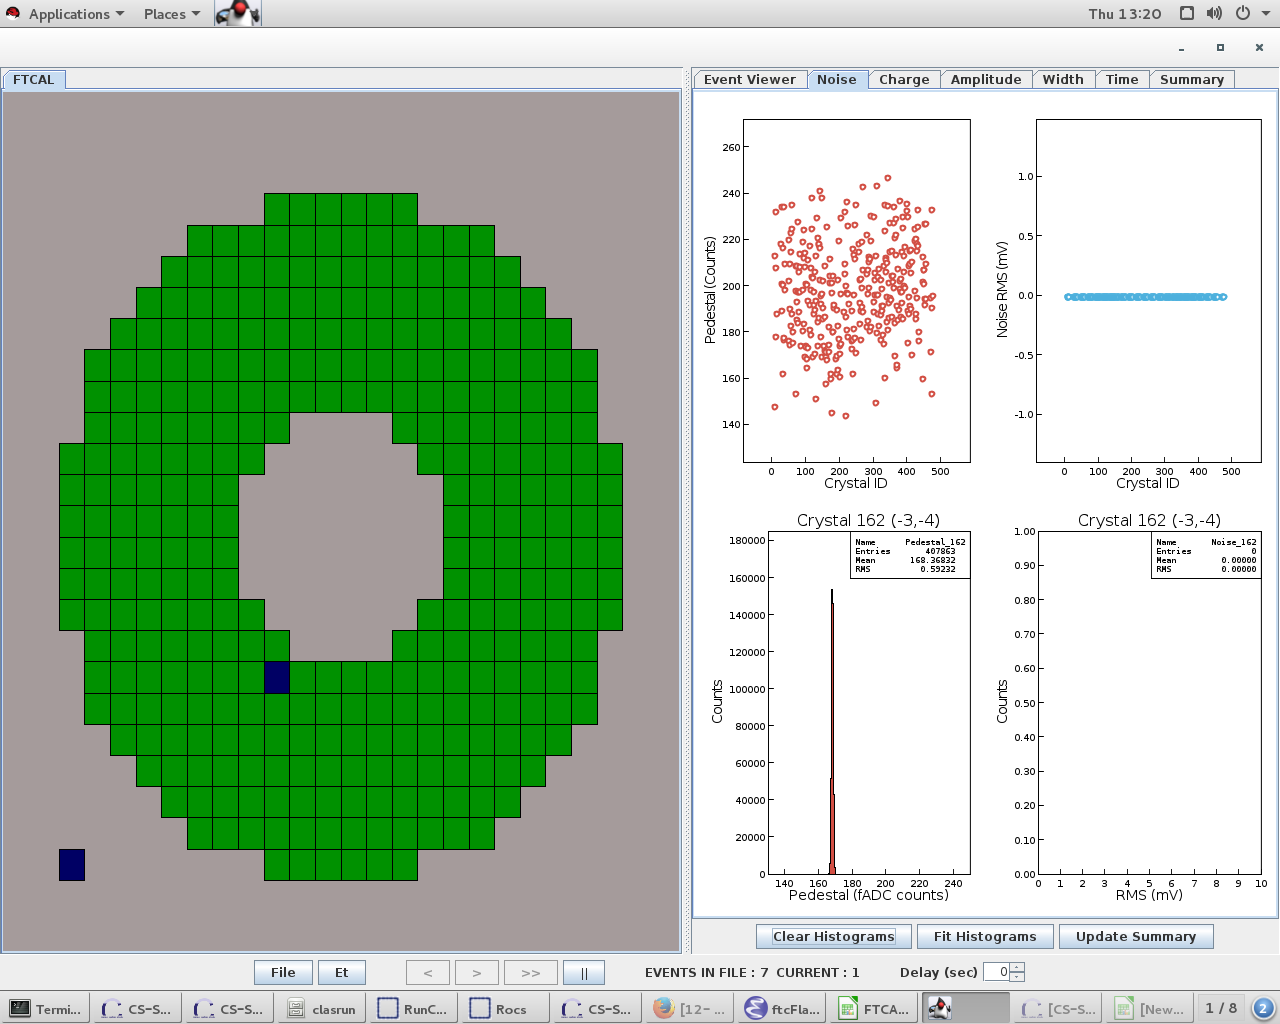
\includegraphics[width=9cm]{pics/NOISE_MAP.png}
    \caption{Example Noise map within the LED monitoring Gui. The color of the heat map is determined by the RMS of the mean of the noise of a given channel.\label{fig:NOISE-MAP}}
\end{figure}
  
\item{If new problematic channels are found, contact the FT-Cal expert on call.}
\end{itemize}
\item{\textbf{Stop the DAQ:} click on ``End Run''. }
\item{\textbf{Stop the LED controller:} end the sequence by clicking on ``Stop'' and turn off the drivers by clicking on ``OFF''. }
\end{enumerate}

When the detector will be installed and the conditions DB defined, instructions on how to upload results will be added to this manual.



\newpage

   \section{Taking a Cosmic Calibration Run}
\begin{enumerate}
\item{\textbf{Start the DAQ system: }}
\begin{itemize}
\item Identify the machine where the DAQ RunControl is running. If you can't find it anywhere, it is possible the DAQ system has to be initialized from scratch. To do so, refer to the CLAS12 DAQ manual, or contact the DAQ expert.
\item Depending on the DAQ state, different buttons may be visible in the ``Transition'' area. If the ``Configure'' button is not visible, click on ``Reset'', then on ``OK''.
\item Click on ``Configure'' to properly set up the run. A ``Run Type Configuration'' dialog will show up. Use the scroll-down menu to select as RunType: FT. This configuration will also save any data on tape. Use instead: FT\_NOER to not save data on tape. ~\ref{fig:SELFTRIG1}

%\%\%\%\%\%\%\%\%\%\%\%\%\%\%\%\%\%\%\%\%\%\%\%\%\%\%\%\
\begin{figure}[htbp]\centering
     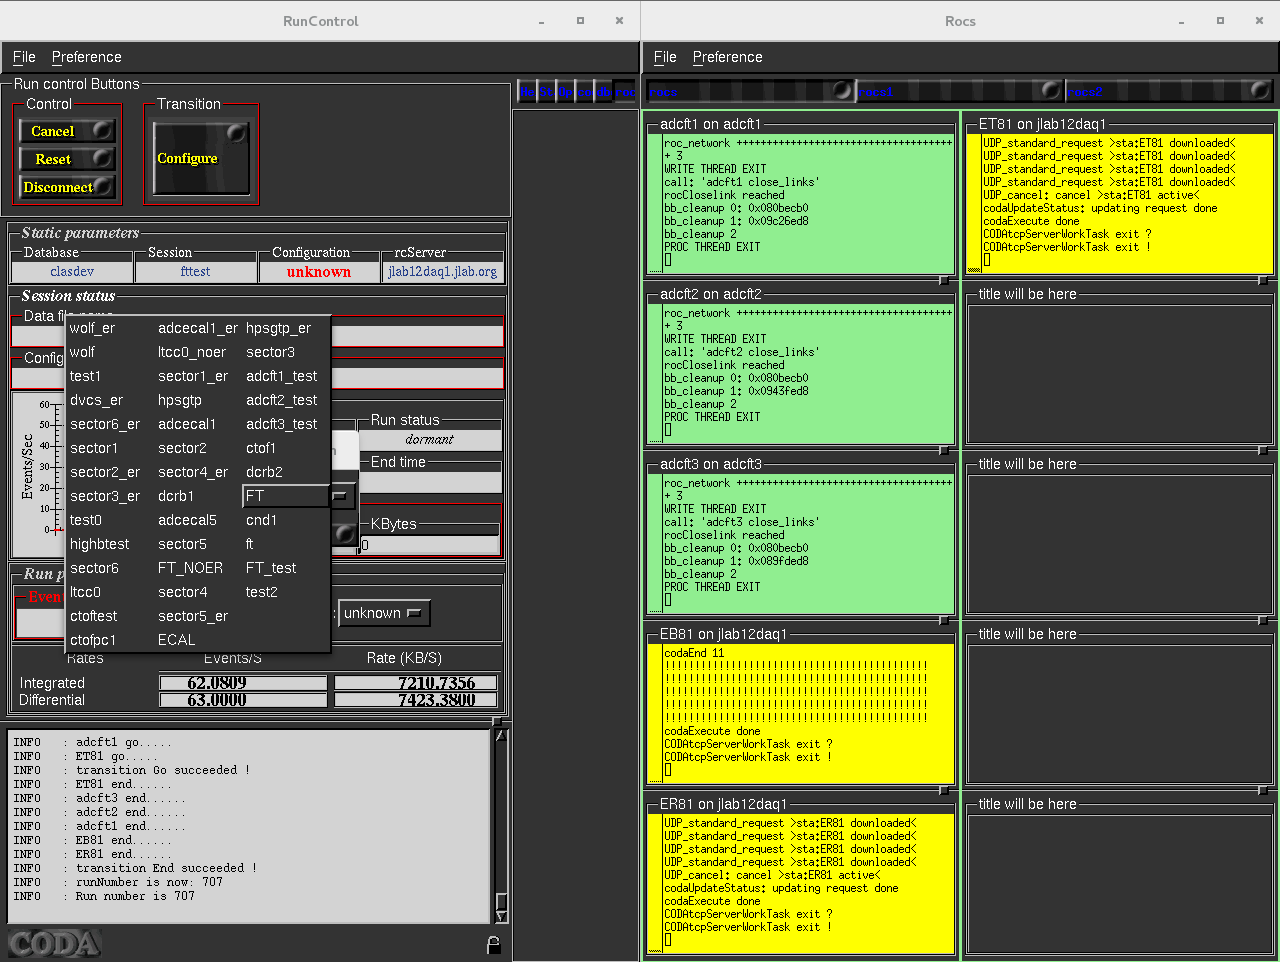
\includegraphics[width=15cm]{pics/SELF_TRIGGER_0.png}
     \caption{Depending on whether the user would like to record or only view live data, there are two configuration options to choose from. The FT option records data, and the FT\textunderscore NOER option only shows live events. \label{fig:SELFTRIG1}}
\end{figure} 
%\%\%\%\%\%\%\%\%\%\%\%\%\%\%\%\%\%\%\%\%\%\%\%\%\%\%\%\


\textit{Default is to save data to the tape}
\item{Click on ``Download'' button. A file-chooser menu will show up.
  On the Left pane of the popup window select .../parms/trigger/FT
  Once within the aforementioned directory Select ft\_selftrigger.trg in the Right pane

  Click on ``OK'' to close the file-choose menu. \ref{fig:SELFTRIG2}}

%\%\%\%\%\%\%\%\%\%\%\%\%\%\%\%\%\%\%\%\%\%\%\%\%\%\%\%\
\begin{figure}[htbp]\centering
  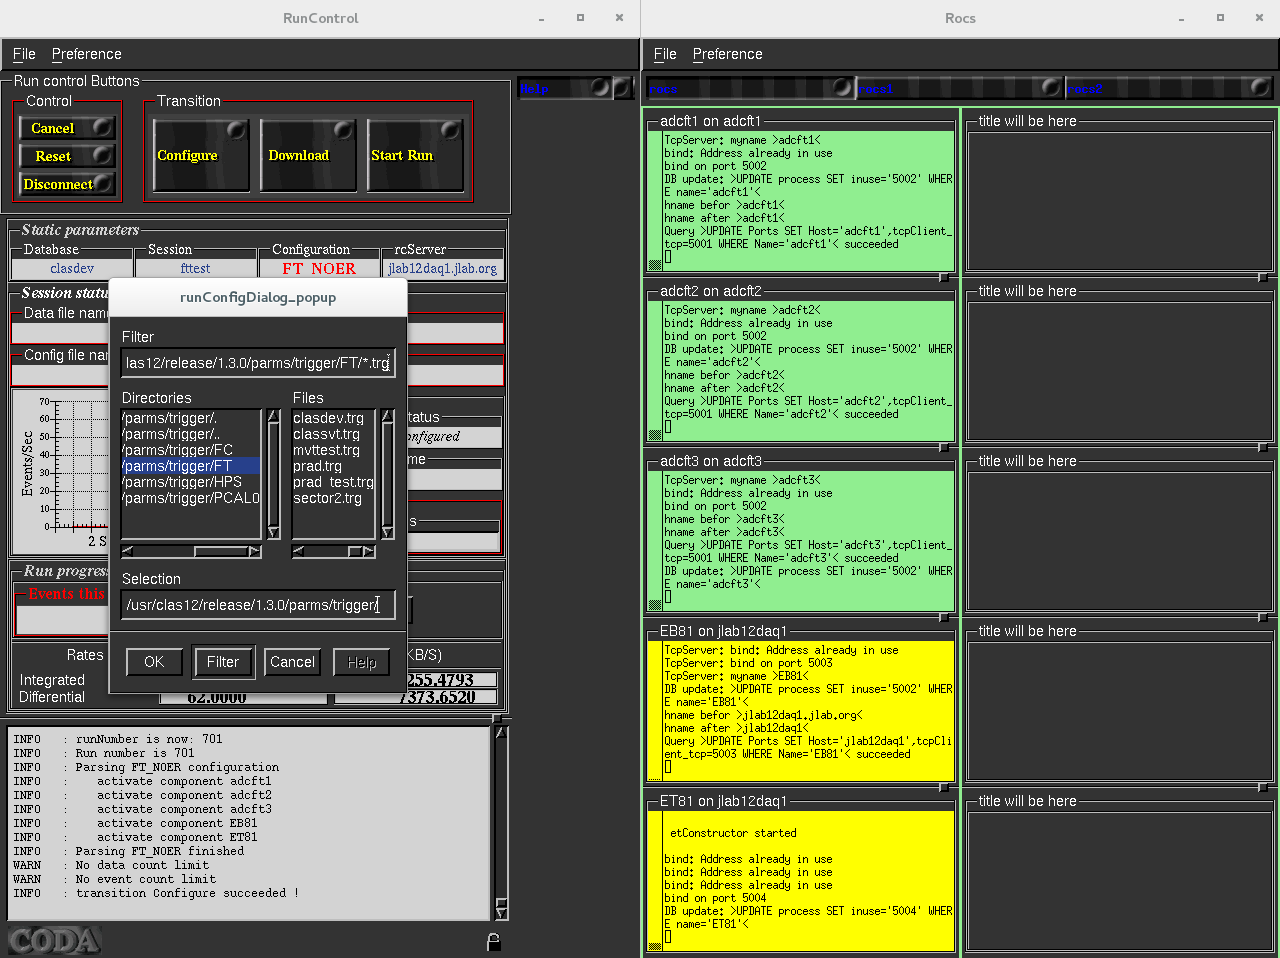
\includegraphics[width=15cm]{pics/SELF_TRIGGER_1.png}
  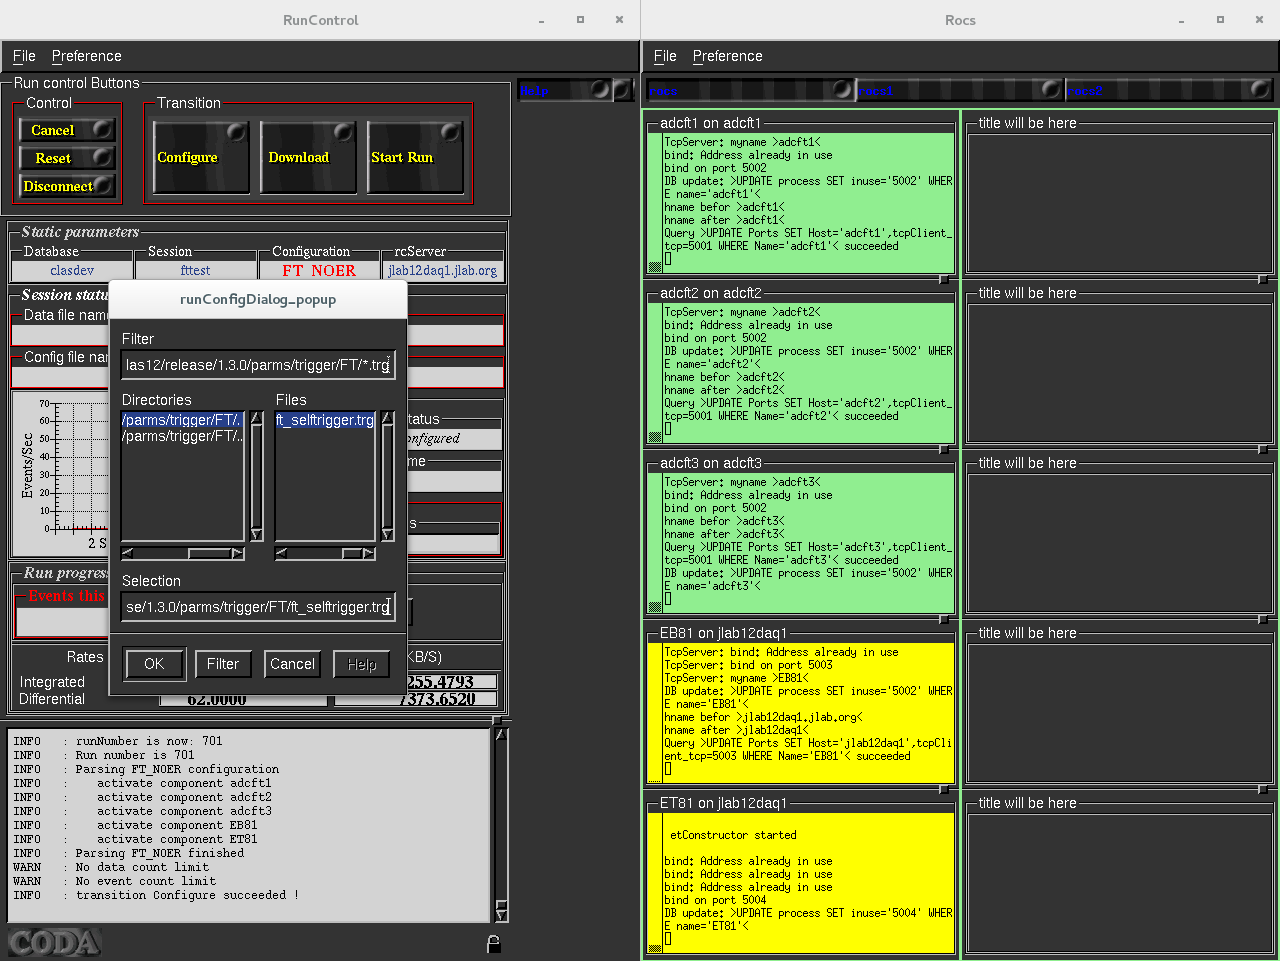
\includegraphics[width=15cm]{pics/SELF_TRIGGER_2.png}
     \caption{Once the configuration has been chosen, the user will then download the corresponding trigger file. In the case of the Forward Tager, this file is accessed by clicking the download button and navigating to .../parms/trigger/FT/ in the left window of the popup, and selecting the file called ft\textunderscore selftrigger.trg in the right window.
       \label{fig:SELFTRIG2}}
\end{figure} 
%\%\%\%\%\%\%\%\%\%\%\%\%\%\%\%\%\%\%\%\%\%\%\%\%\%\%\%\

\item{Click on ``Prestart''.  Wait until the ``GO'' button appears.}
\item{In the RunControl GUI, click on the ``GO'' button. Wait 10~s, until the message ``transition go succeded'' is displayed in the log window and the ``END'' button displays.}
\end{itemize}
\item{\textbf{Start the monitoring app: }}
\begin{itemize}
\item{Use the command outlined in the previous section to start the monitoring app. When the monitoring gui window shows up, click on the ``Et'' button to connect to the ET ring and on the ``$>>$ button to start the event processing. }
\item{Once connected to the ET ring the user will see live events on the Left pane of the monitoring app\ref{fig:CROSSING}, as well as the waveform and tabs to provide further analysis on the Right.}
\end{itemize}

\begin{figure}[htbp]\centering
  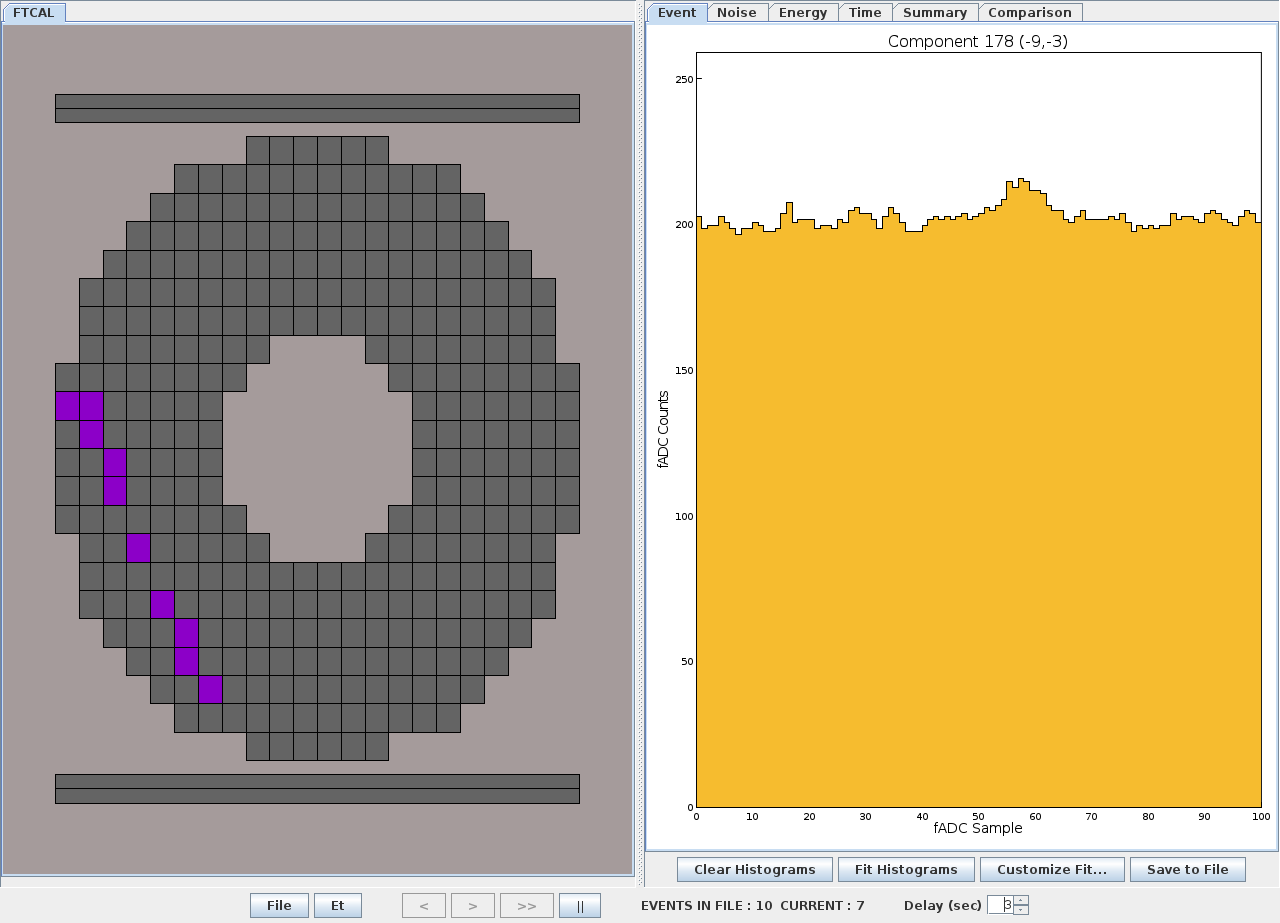
\includegraphics[width=15cm]{pics/Success_Successo.png}
     \caption{Sample cosmic event showing the channels being activated, as well as a histogram for a selected channel, which shows read waveform.}
       \label{fig:CROSSING}
\end{figure}

\end{enumerate}
\newpage
%\%\%\%\%\%\%\%\%\%\%\%\%\%\%\%\%\%\%\%\%\%\%\%\%\%\%\%\

\iffalse
   \section{Taking a Pedestal Run}
\textcolor{red}{we should check with Sergey about this procedure both for beam and no beam}

   \subsection{With Beam}
   Pedestals are calculated at running luminosity with DAQ configuration \begin{center}\texttt{ecalPedestal.trg}\end{center} and monitored and analyzed with HPS's hps-java monitoring app via the command:
       \begin{center}\texttt{startEcalPedestalCalculator}\end{center}
       In this monitoring app you can click on the event display to view the different channels' pedestal histograms as the data is acquired.  Once the statistics are sufficient, the app should be disconnected from the ET-ring and then output files for the DAQ and database will be generated in the directory:\begin{center}\texttt{\$HOME/EcalPedestals}\end{center}  The user will be asked if they want them put in the database automatically, and it requires two consecutive ``YES'' responses to make it happen.  An expert should make the trigger configuration use the new pedestal file.

         \subsubsection{Installing the new pedestals}
      To generate the pedestal file for the DAQ, run this script, where the last argument is the name of the file generated in the previous step:
         \begin{center}\texttt{calibUtilHpsEcal.py -P -DAQ -N -b XYZ\_hpsDB.txt}\end{center}

  \subsection{Without Beam}
  Coming soon.
\fi

\newpage

\part{FT-Cal Experts Resources}

   \section{Location of FT-Cal Ancillary Systems}

   {\footnotesize
\begin{itemize}
\item
The chiller is located beam-right on Level 2 space frame.~\ref{fig:ChillBro}
\item
The LED controllers are located in the FT racks under the subway. See Figure~\ref{fig:LEDcontroller}.
\item
The FADCs and patch panels occupy the top part of the FT racks under the subway. See Figure~\ref{fig:FADC}.
\item
    The HV supply is located beam-left on Level 1 space frame.  See Figure~\ref{fig:HVPHOTO}.
\item
    The LV supply is located in the FT racks under the subway. See Figure~\ref{fig:LVPHOTO}.
\end{itemize}
The layout of the FT racks (located under the subway) is shown in Fig.~\ref{fig:ft-elec-lo}.
   }%\%\%\%\%\%\%\%\%\%\%\%\%\%\%\%\%\%\%\%\%\%\%\%\%\%\%\%\

\begin{figure}[htbp]\centering
    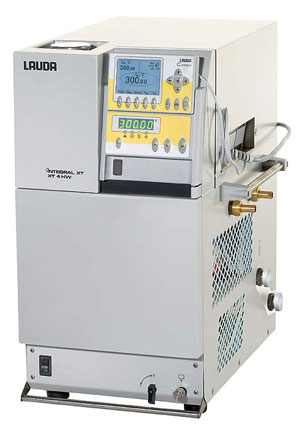
\includegraphics[width=7cm]{pics/LAUDA_XT150.jpg}
    \caption{LAUDA XT150 chiller will be located beam-right on Level 2 space frame.\label{fig:ChillBro}}
\end{figure}

\begin{figure}[htbp]\centering
    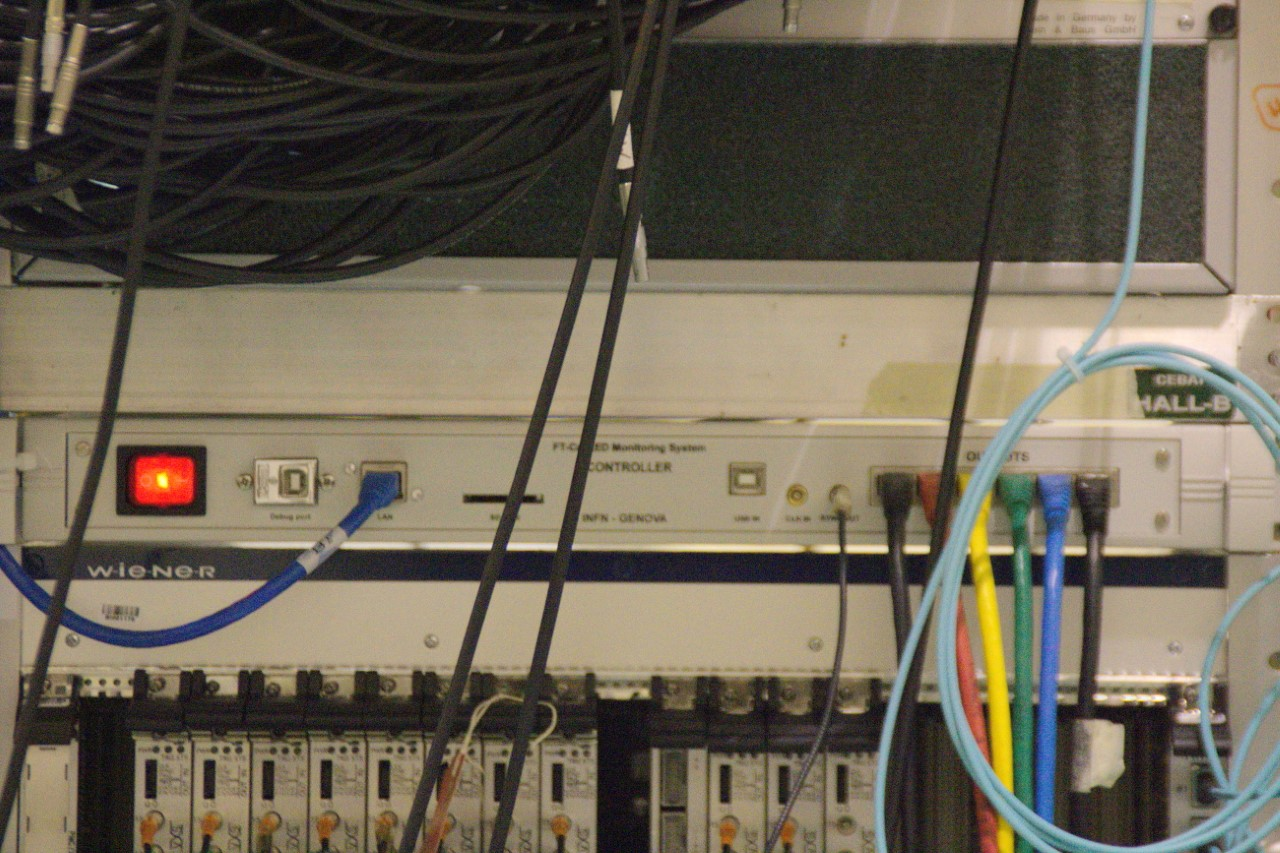
\includegraphics[width=7cm]{pics/LED_FLASHER.jpg}
    \caption{LED flasher controller located in the FT racks under the subway.\label{fig:LEDcontroller}}
\end{figure}

\begin{figure}[htbp]\centering
    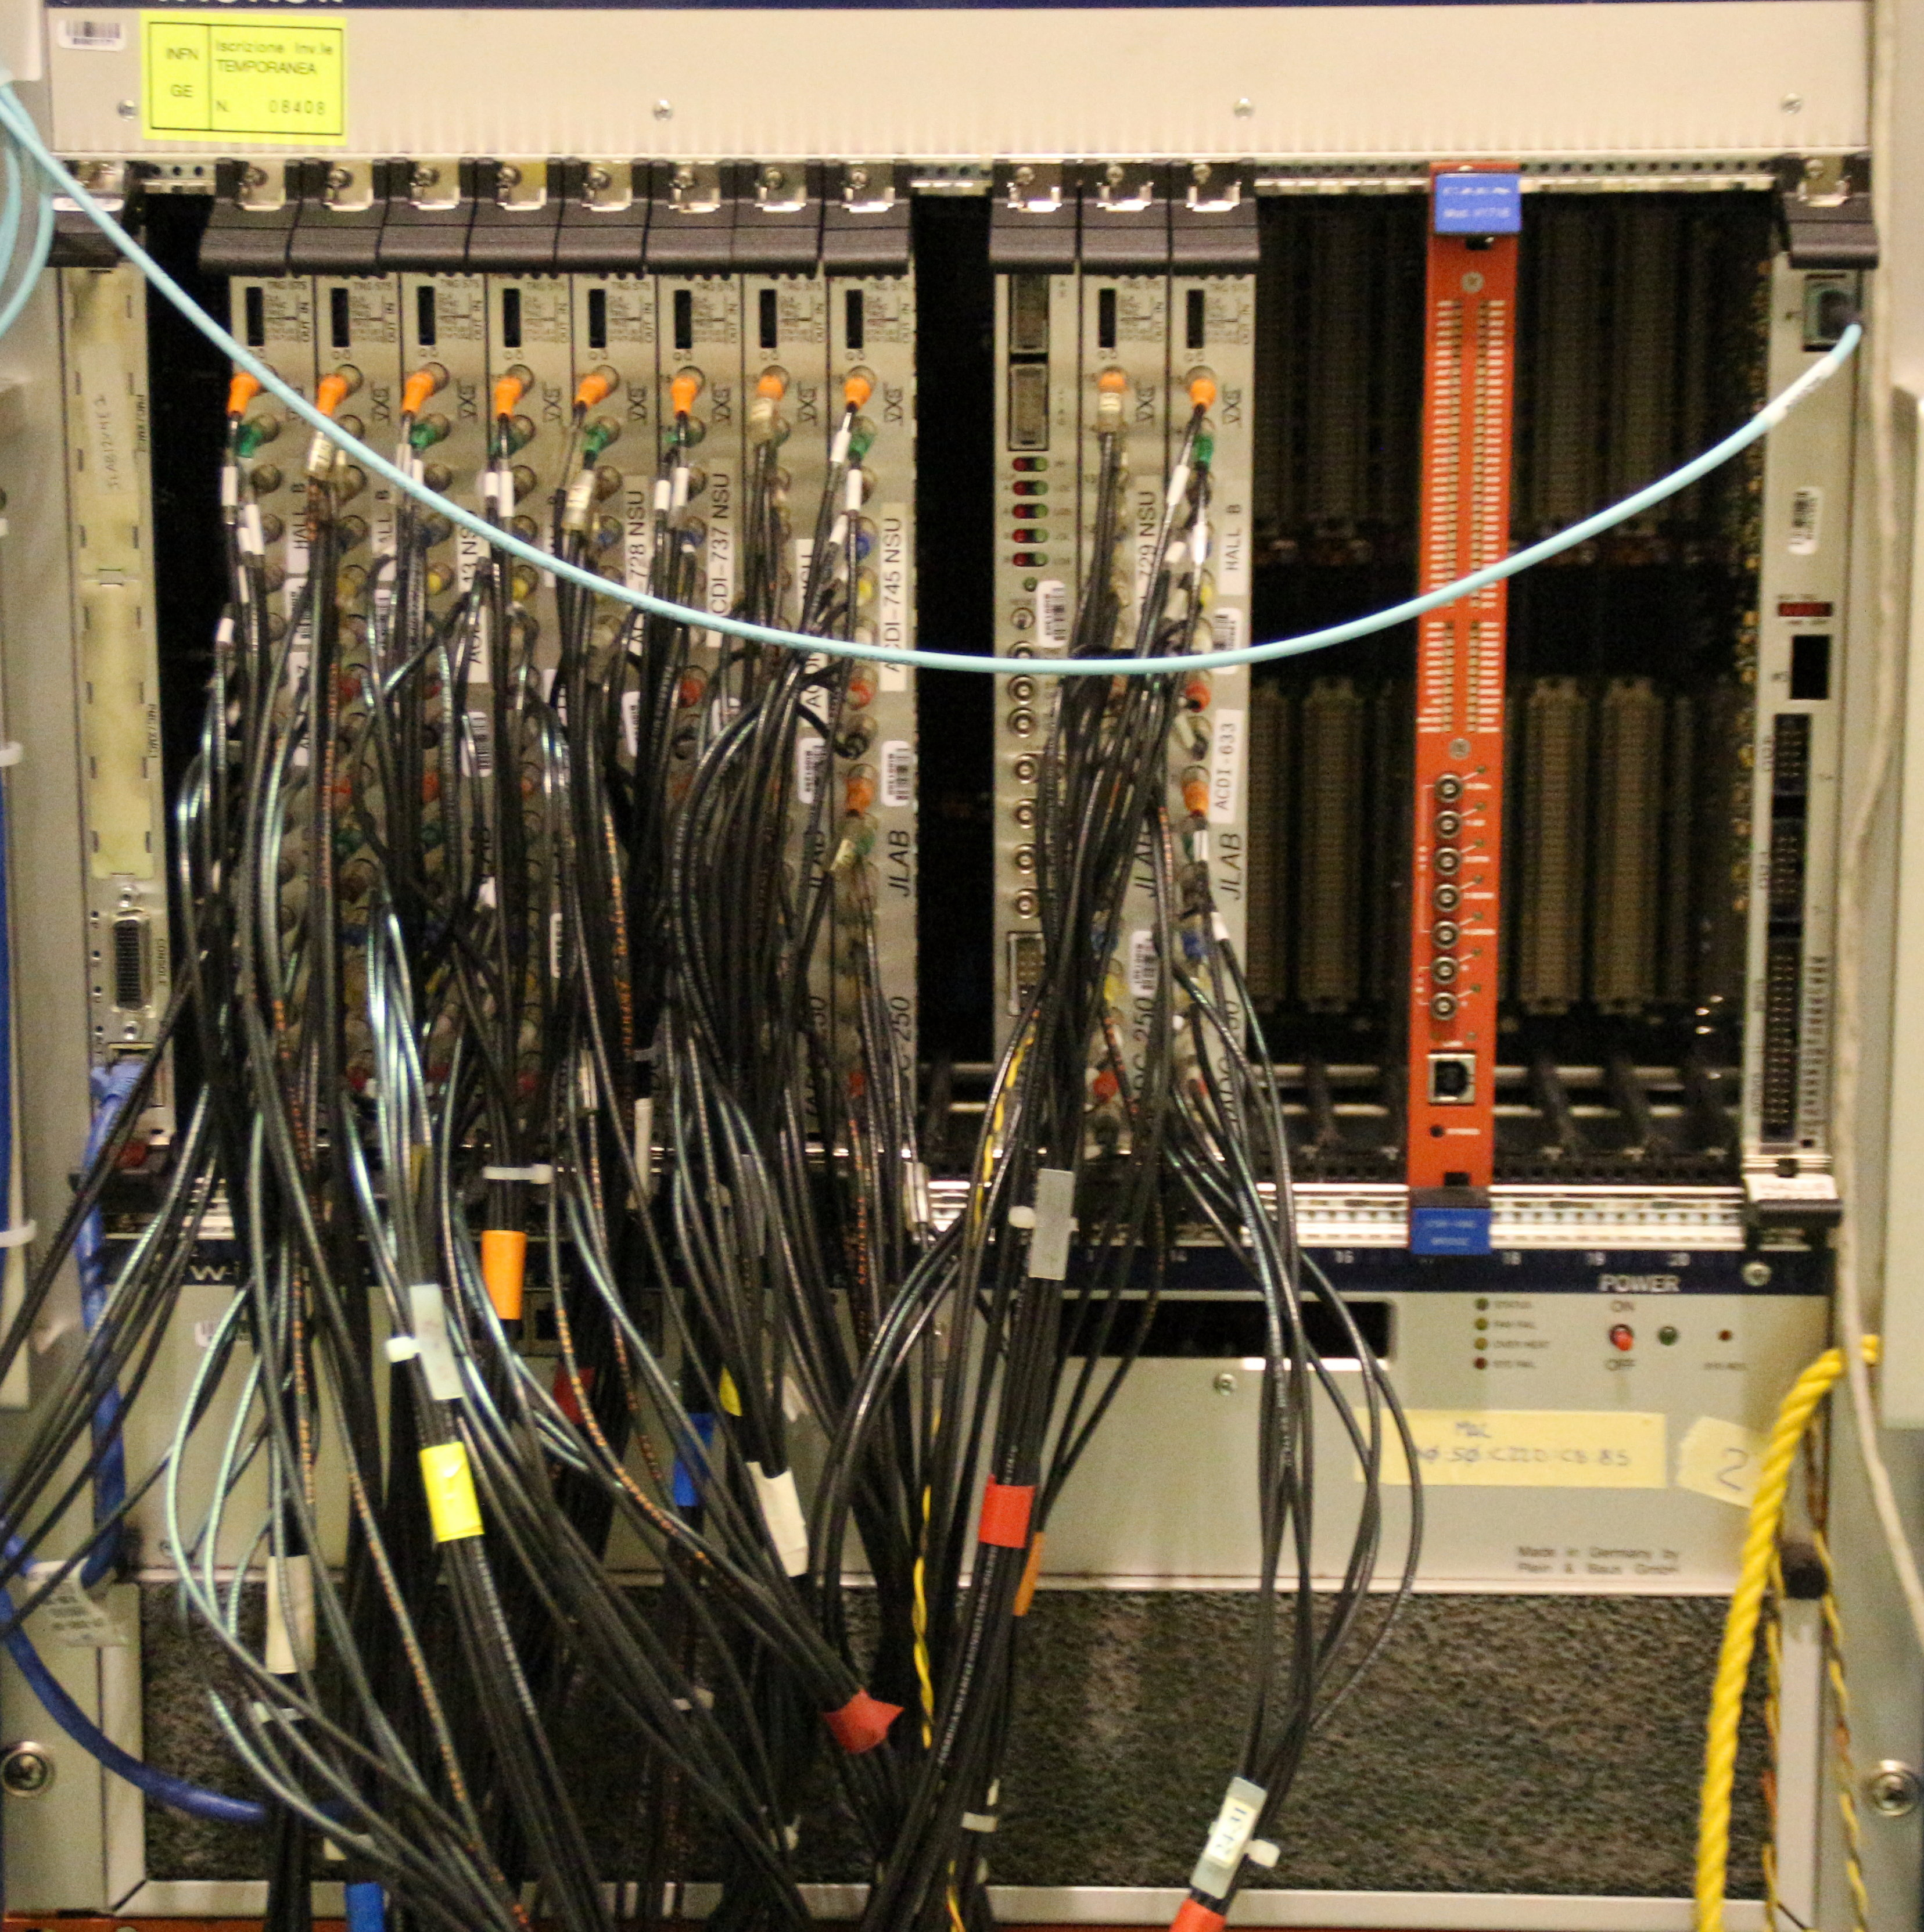
\includegraphics[width=7cm]{pics/FADC_CRATE.jpg}
    \caption{One of the FADC crates for the Forward Tagger located in the racks under the subway.\label{fig:FADC} {\em To be replaced with a picture of the fADC rack in the Hall.}}
\end{figure}
   
\begin{figure}[htbp]\centering
    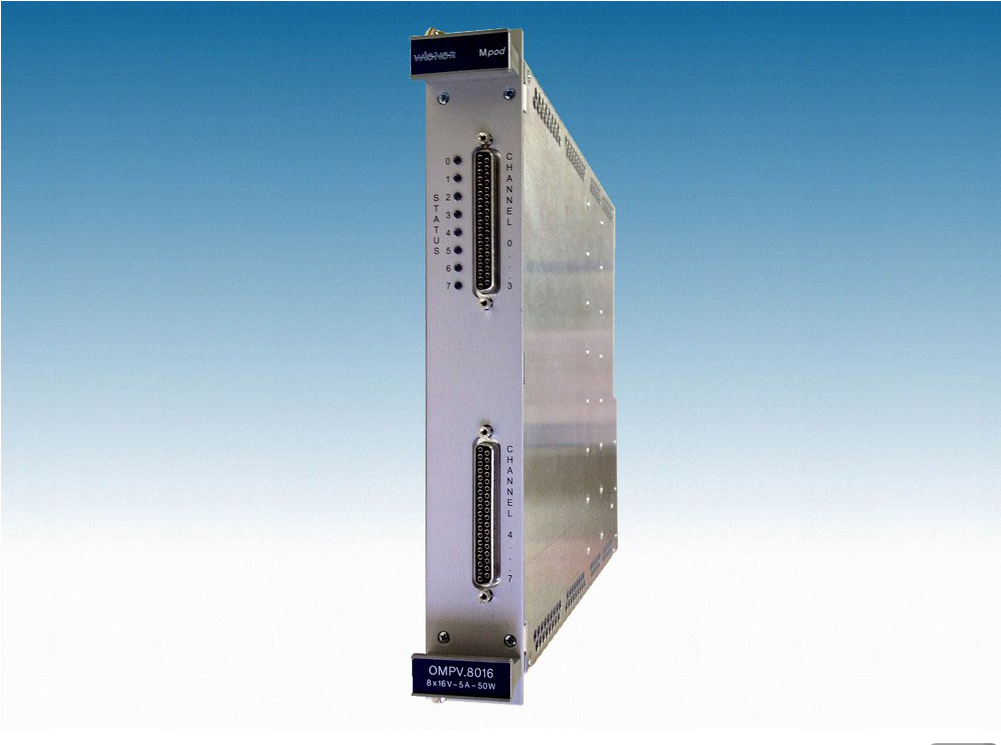
\includegraphics[width=7cm]{pics/LV_OMPV_8008_BOARD.png}
    \caption{MPOD crate containing the OMPV.8008 LV supply board located in the FT racks under the subway.\label{fig:LVPHOTO}}
\end{figure}

\begin{figure}[htbp]\centering
    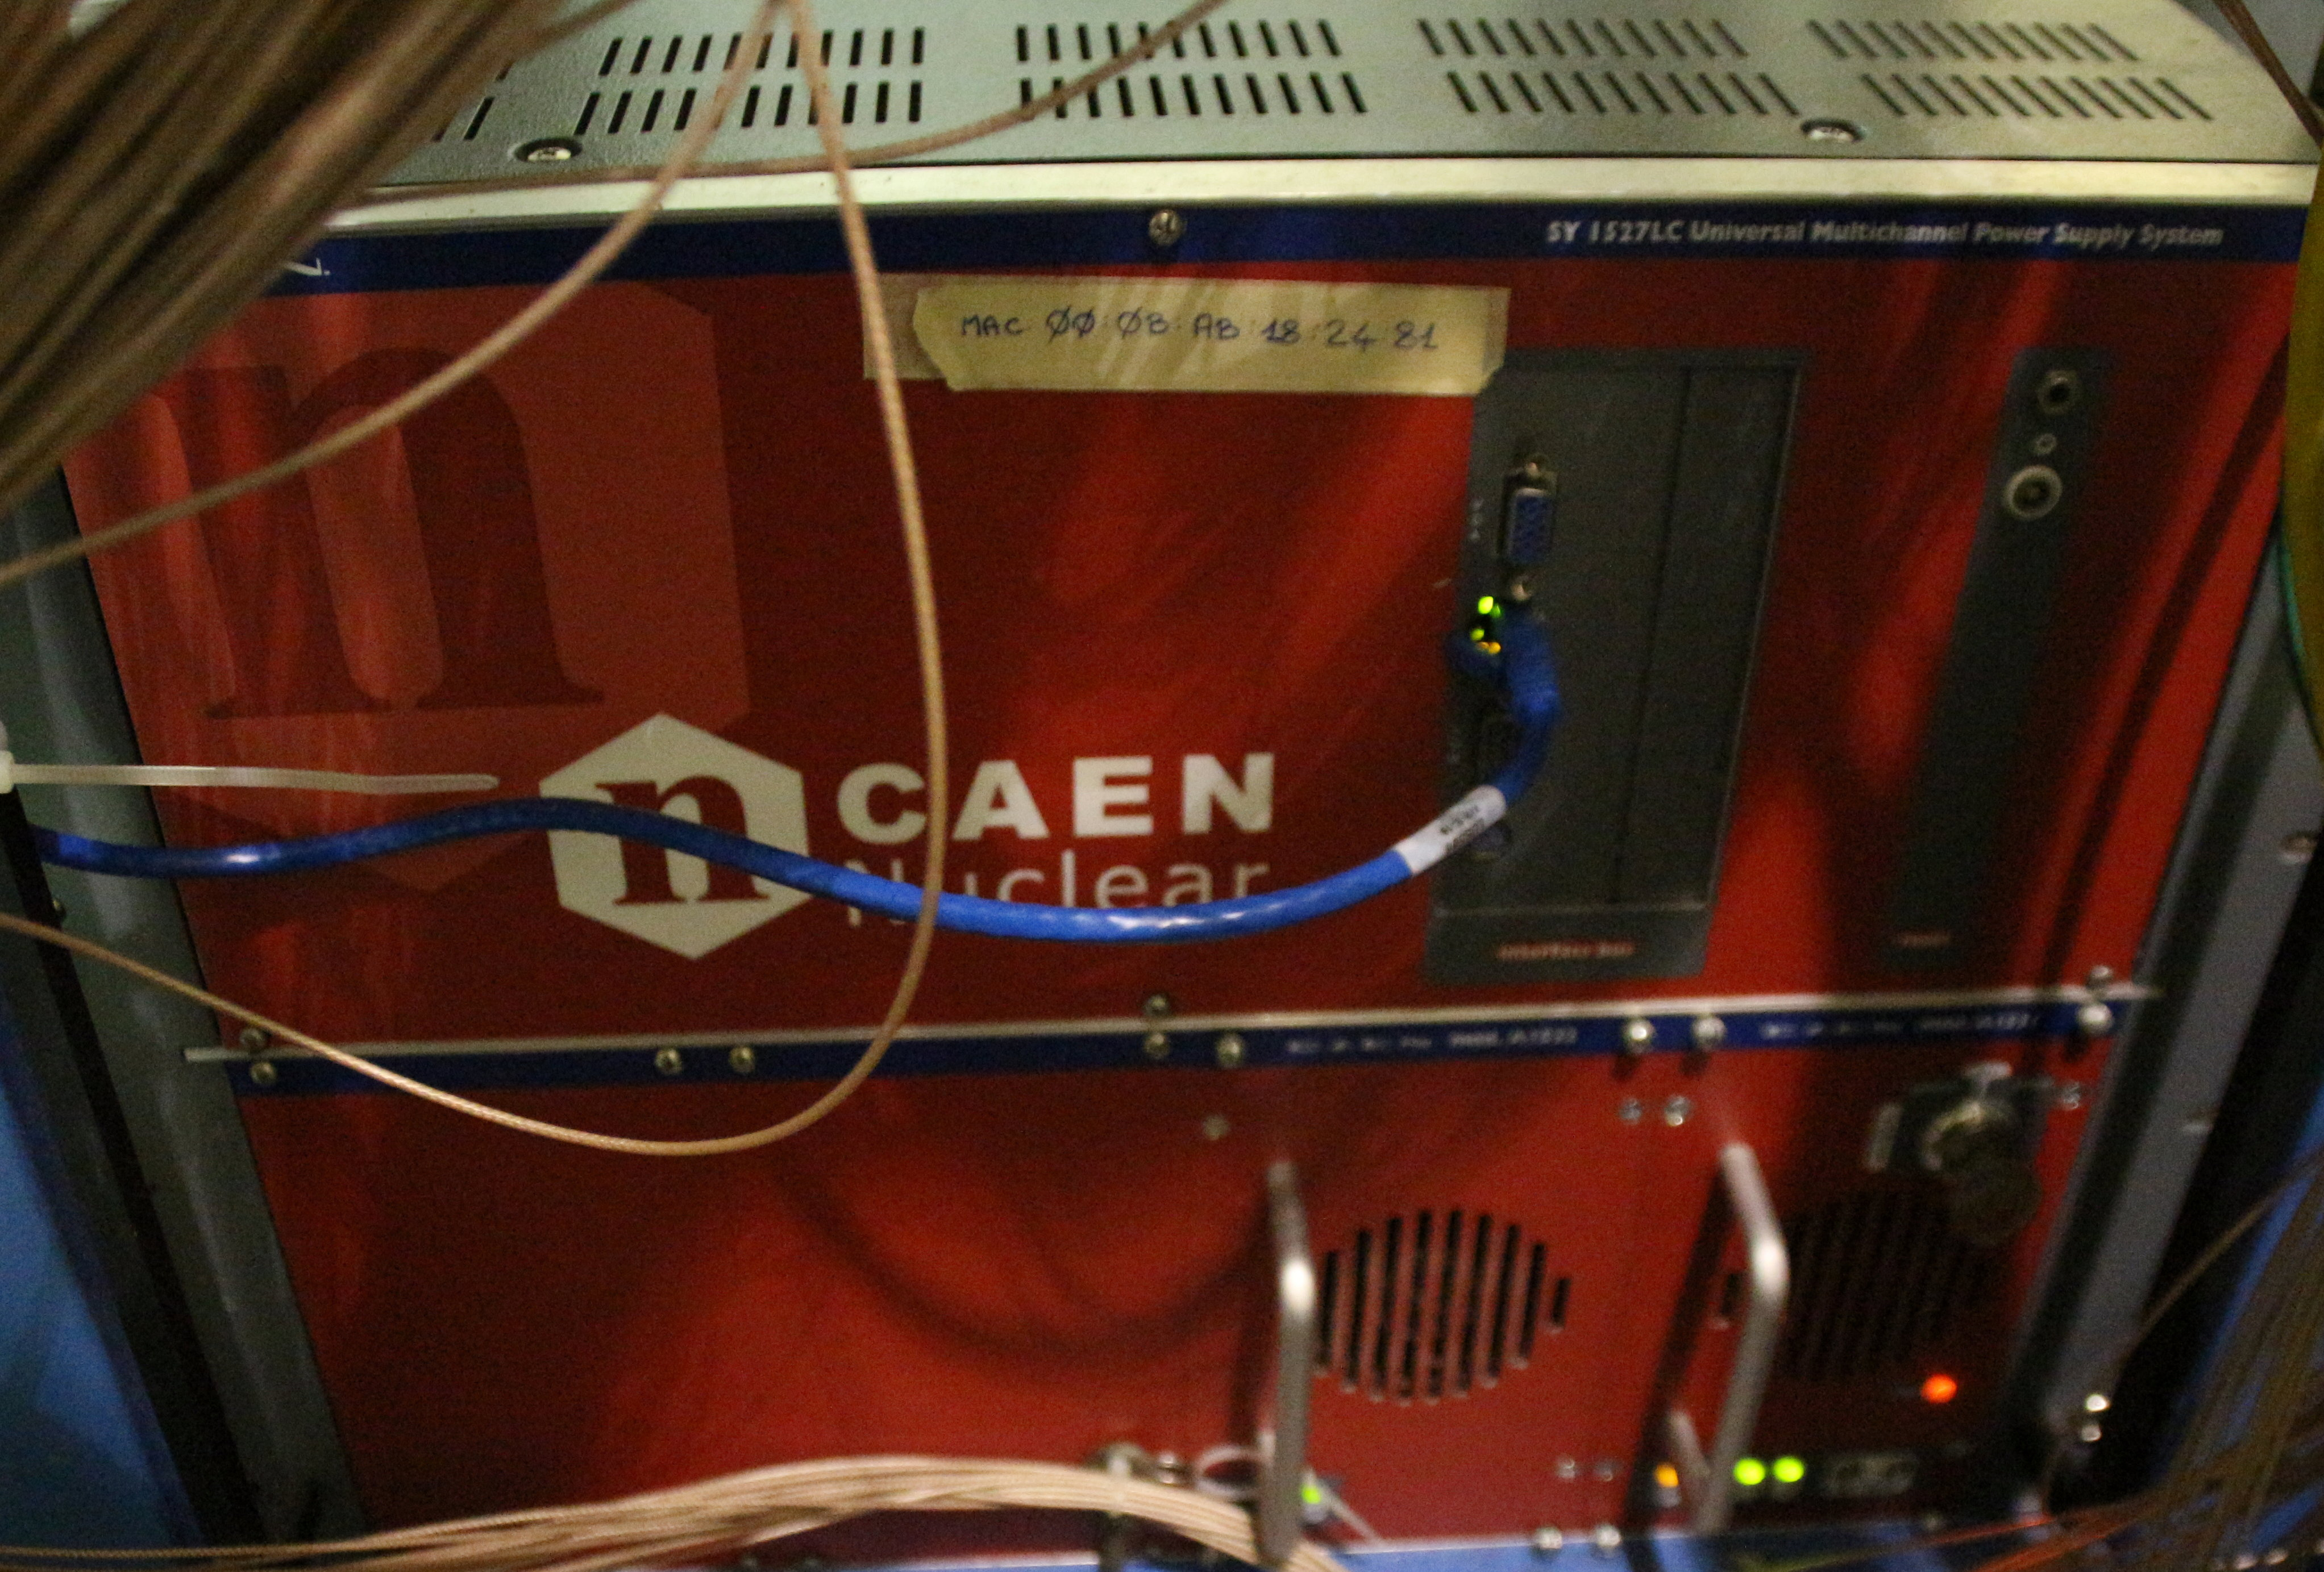
\includegraphics[width=9cm]{pics/CAEN.jpg}
    \caption{CAEN  HV power supply located on the beam-left side of Level 1 Space Frame.  Key for on/off is in the lower right corner of the crate.\label{fig:HVPHOTO}}
\end{figure}

\begin{figure}[htbp]\centering
    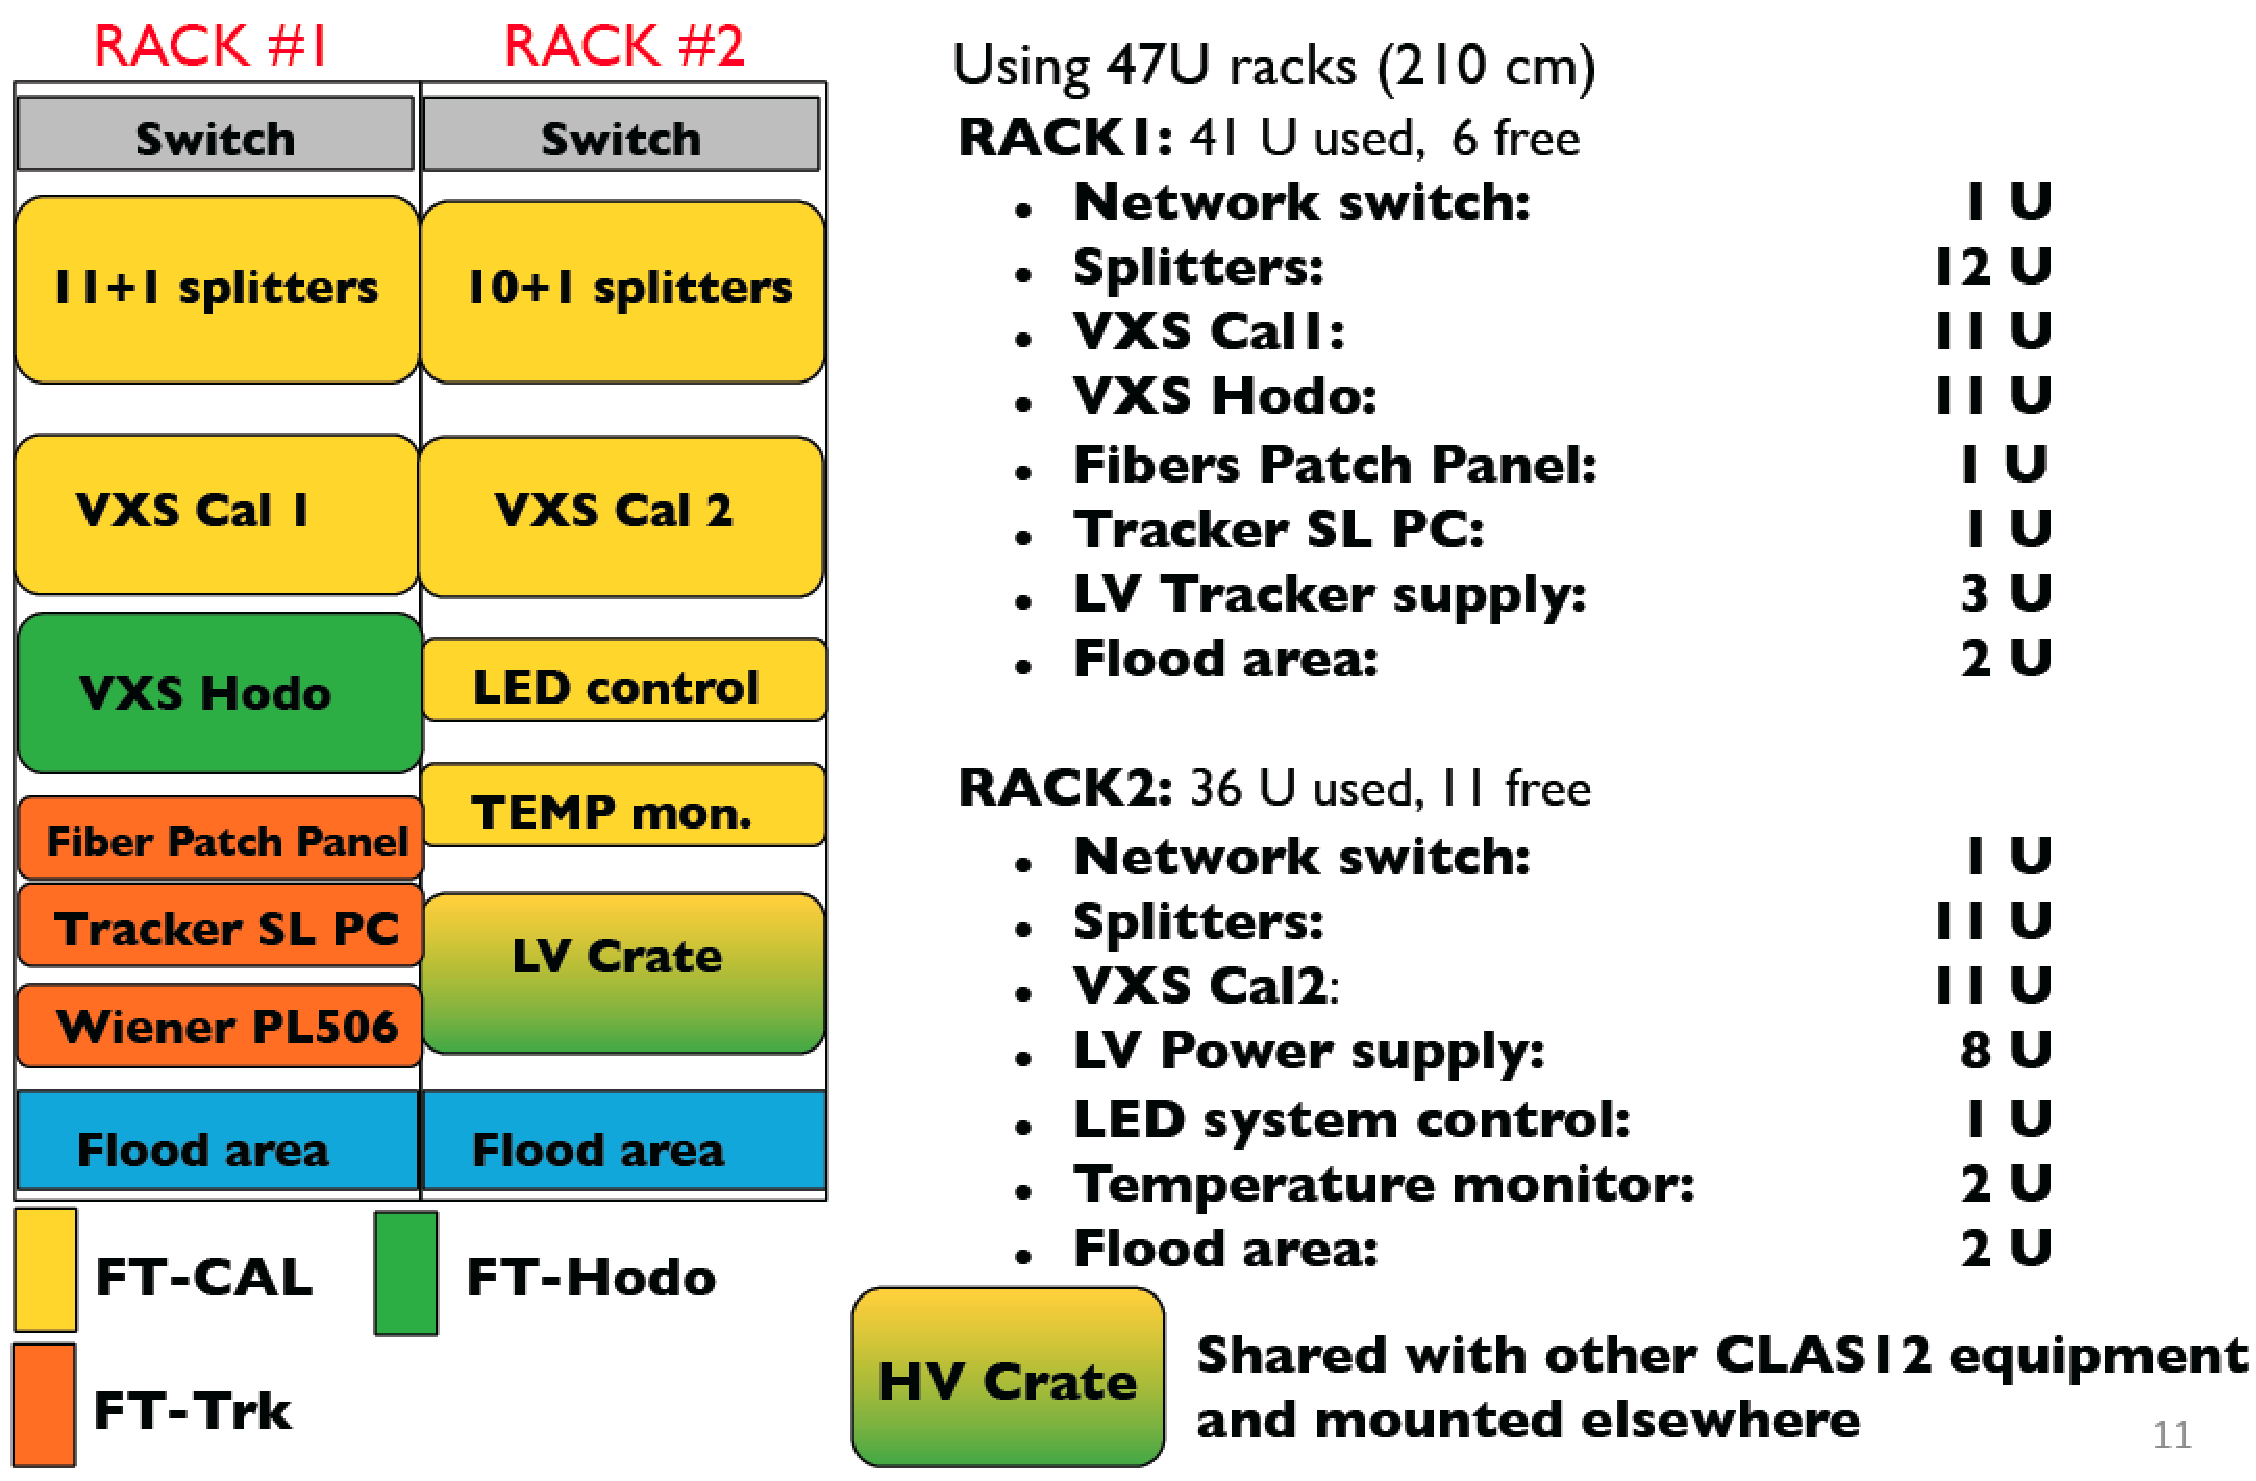
\includegraphics[width=15cm]{pics/ft-elec-lo.pdf}
    \caption{FT electronic racks layout.\label{fig:ft-elec-lo}}
\end{figure}
 

%\%\%\%\%\%\%\%\%\%\%\%\%\%\%\%\%\%\%\%\%\%\%\%\%\%\%\%\
% \newpage
%    \section{Cooling system}

%    The cooling system is using an ANOVA A-40 chiller that can be controlled through EPICS (\ref{ChillerCam}). The setting should not be modified; the temperature setting should be fixed at 17 degrees Celsius.  If any of the readbacks in our EPICS screens for these systems are empty and white, it may be necessary to reboot the corresponding IOC. 
%    %In case of problem with the chiller contact ??? (who can take care of these in Hall-B engineer group?).  
%    %The manual for the chiller can be found here:
%    %{\noindent\footnotesize\url{http://www.nist.gov/ncnr/upload/Circulating-Bath\_Thermo-Scientific\_NESLAB-RTE-7.pdf}}
%      \subsection{Rebooting the Chiller After Power Failure}
%      {\em This section applies to the old Thermo-Scientific chiller that was replaced in April 2015.  We have not had the opportunity to experience how the new ANOVA A-40 chiller responds to a power failure while in remote mode.}

%      If the chiller loses power while in local mode, the ``power'' button must be pressed manually to restart it after power is restored.  In case it loses power while in remote mode, a procedure is necessary to reset it after power is restored:
%    {\footnotesize
%      \begin{enumerate}
%          \item Hold the ``up'' and ``down'' arrow buttons simultaneously for 10 seconds.
%          \item Press the ``computer'' button to go into local mode.
%          \item Press the ``power'' button to turn it off.
%          \item Press the ``power'' button to turn it on.
%          \item Press the ``computer'' button to return to remote mode.
%     \end{enumerate}
%     }

%     \subsection{Restarting the Chiller IOC}
%     Chiller IOC runs in ``procserv'', a wrapper that automatically runs and restarts services and provides access to them via telnet.  To restart the chiller's IOC:
%    {\footnotesize
%    \begin{enumerate}
%        %\item \texttt{`ssh hpsrun@clonsl1'}
%        \item \texttt{`softioc\_console iocchiller'} and type user's password if necessary.
%        \item \texttt{`ctrl-x'} to restart the IOC
%        \item \texttt{`ctrl-]'} to quit to telnet
%        \item \texttt{`quit'} to exit telnet
%    \end{enumerate}
%    }
% \noindent{\em Don't leave a terminal open connected to this telnet session.}

%    \subsection{Restarting the Temperature Monitoring IOC}
%    Thermocouples are used to monitor the temperature inside and outside the calorimeter.  To restart the IOC that reads these:
%    {\footnotesize
%    \begin{enumerate}
%        %\item \texttt{`ssh hpsrun@clonsl1'}
%        \item \texttt{`softioc\_console ioctempSens'} and type user's password if necessary.
%        \item \texttt{`ctrl-x'} to restart the IOC
%        \item \texttt{`ctrl-]'} to quit to telnet
%        \item \texttt{`quit'} to exit telnet
%    \end{enumerate}
%    }
% \noindent{\em Don't leave a terminal open connected to this telnet session.}


\newpage
   \section{LV Supply}
      The low voltage power supply is an Wiener MPOD OMPV.8008.  It should be set with all four channels at $+5$V with their current limits at 5 A, while external wiring inverts one channel to create a bipolar $\pm5$V supply. 

      The low voltage supply might have difficulties to get to full voltage because of high current for intense beam operation. If that was the case check, with all power supplies off, that all connection are goods. Then contact run coordinator to see if the current limit should be increased. 

\subsection{Changing LV Settings}
The LV supply can be controlled via its EPICS expert screen (Figure~\ref{lvexpert}), accessible from the grey button in the top right of the LV section of the main FT-Cal EPICS screen (Figure~\ref{fig:ecal_all}). In general the only necessary changes are powering on/off, while voltage and current setpoints are never changed from 5V/5A.

%\%\%\%\%\%\%\%\%\%\%\%\%\%\%\%\%\%\%\%\%\%\%\%\%\%\%\%\
\begin{figure}[htbp]\centering
    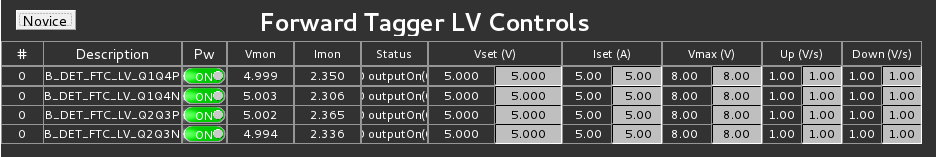
\includegraphics[width=0.9\textwidth]{pics/lvexpert.png}
    \caption{The LV expert EPICS screen in normal operation.\label{lvexpert}}
\end{figure}
%\%\%\%\%\%\%\%\%\%\%\%\%\%\%\%\%\%\%\%\%\%\%\%\%\%\%\%\

{\em Note, as a safeguard, if one currently tries to use EPICS to set the voltage greater than 5 V or the current greater than 5 A, the request will be ignored by the IOC.}  

\newpage
   \section{High Voltage}
   \subsection{Changing HV Settings}
      {\bf NOTE:} Changing voltage settings should be taken care of in coordination with the FT-Cal group (contact M.~Battaglieri). 
%Current setting can be increased by 10\% in case of need, please document this change in the log book and notify the FT-Cal expert on call.

 {\bf NOTE:} The FT-Cal HV groups were renumbered for EPICS, and the correspondence map (Figure~\ref{fig:ExpertMap}) is available on the following webpage: https://logbooks.jlab.org/entry/3370066


%\%\%\%\%\%\%\%\%\%\%\%\%\%\%\%\%\%\%\%\%\%\%\%\%\%\%\%\
\begin{figure}[htbp]
\center
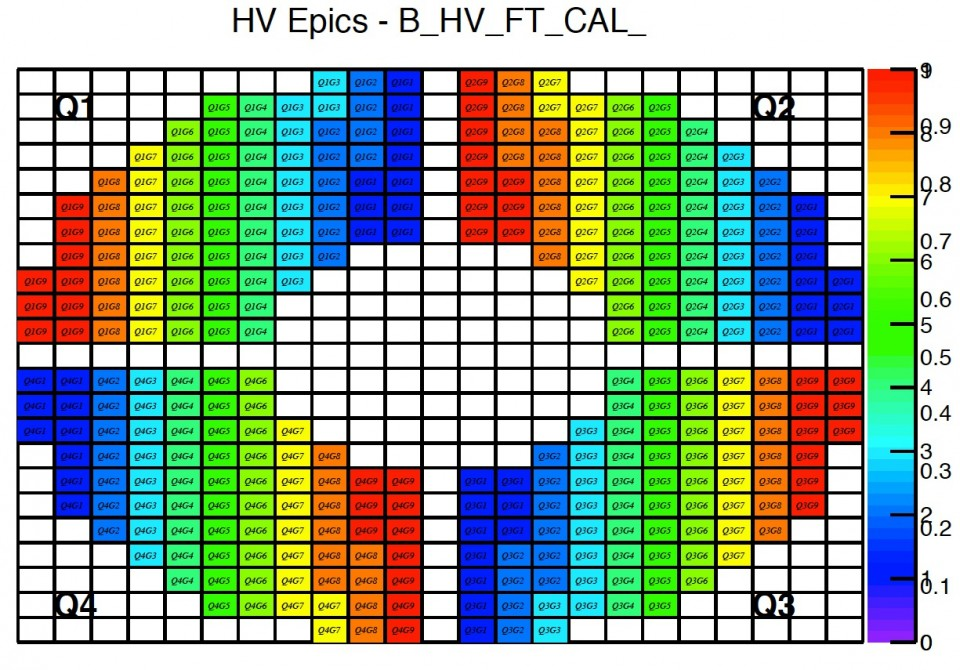
\includegraphics[width=0.95\textwidth]{pics/FT-CalMap.jpg}
\caption{ \label{fig:ExpertMap} HV channel map for reference.}
\end{figure}
%\%\%\%\%\%\%\%\%\%\%\%\%\%\%\%\%\%\%\%\%\%\%\%\%\%\%\%\


      If for some reason some channels were to drop in gain (or increase) or if the current drawn increases in a group, it might be necessary to change the HV settings in the expert FT-Cal EPICS control (Fig.~\ref{fig:HVControl}). A modification of the voltage will lead to a modification of the gain used by the trigger system, these values need to be updated at the same time!

\newpage    
      \subsubsection{HV Save/Restore}
      A system to save and restore the entire calorimeter's voltage settings is available via the grey button in the HV section of the main Overview page, shown in Figure~\ref{fig:ecal_all}.  If the voltage setpoints are changed, a backup should be made of the new settings.  This must be run as clasrun user in directory  \texttt{/usr/clas12/DATA/burt/FTC\_HV}.
      An example of the restore window is shown in Figure~\ref{fig:hvrestore}, which is accessible from the FTC Overview screen shown in Figure~\ref{fig:ecal_all}.

%\%\%\%\%\%\%\%\%\%\%\%\%\%\%\%\%\%\%\%\%\%\%\%\%\%\%\%\
\begin{figure}[htbp]
\center
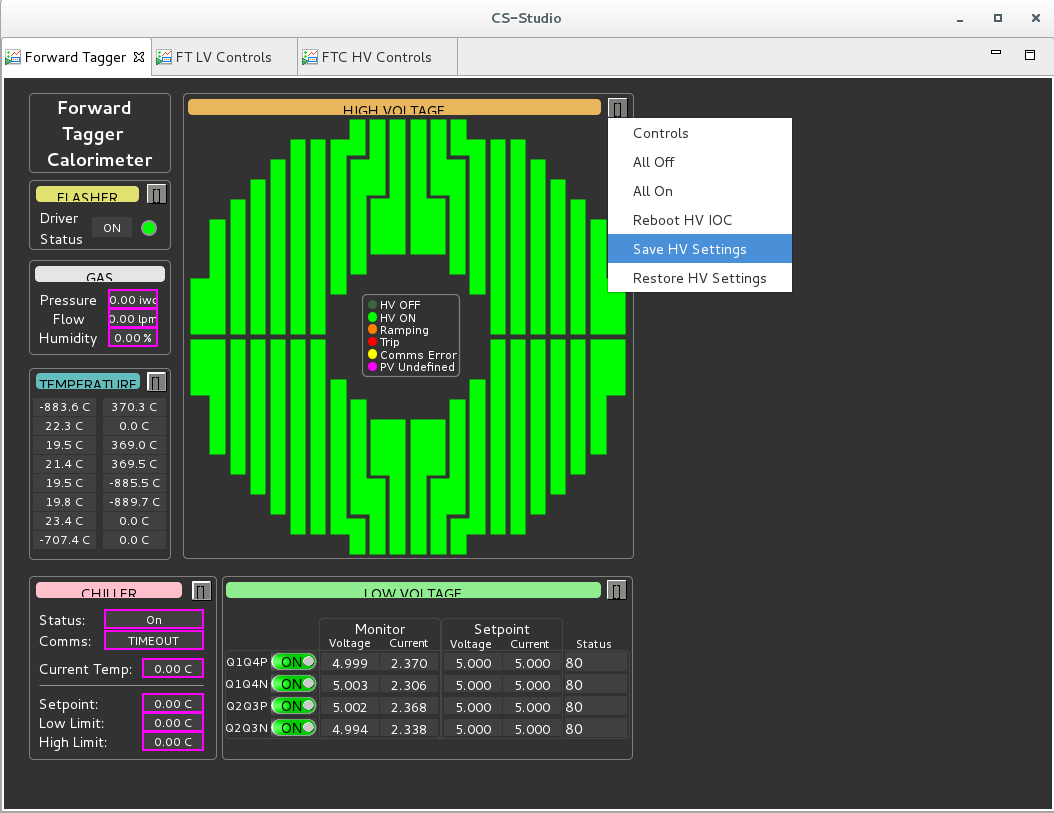
\includegraphics[width=0.85\textwidth]{pics/HVsave_restore.png}
\caption{\label{fig:hvrestore} Menu button within the High Voltage section of the FTC Overview window which allows the user to save HV setting. To restore simply use the next option below, within the same menu.}
\end{figure}
%\%\%\%\%\%\%\%\%\%\%\%\%\%\%\%\%\%\%\%\%\%\%\%\%\%\%\%\

\section{Channel Mapping GUI}
Channel mapping is available as Annex to this manual.

\newpage

\section{LED system for experts}


%\%\%\%\%\%\%\%\%\%\%\%\%\%\%\%\%\%\%\%\%\%\%\%\%\%\%\%\
\begin{figure}[htbp]
\center
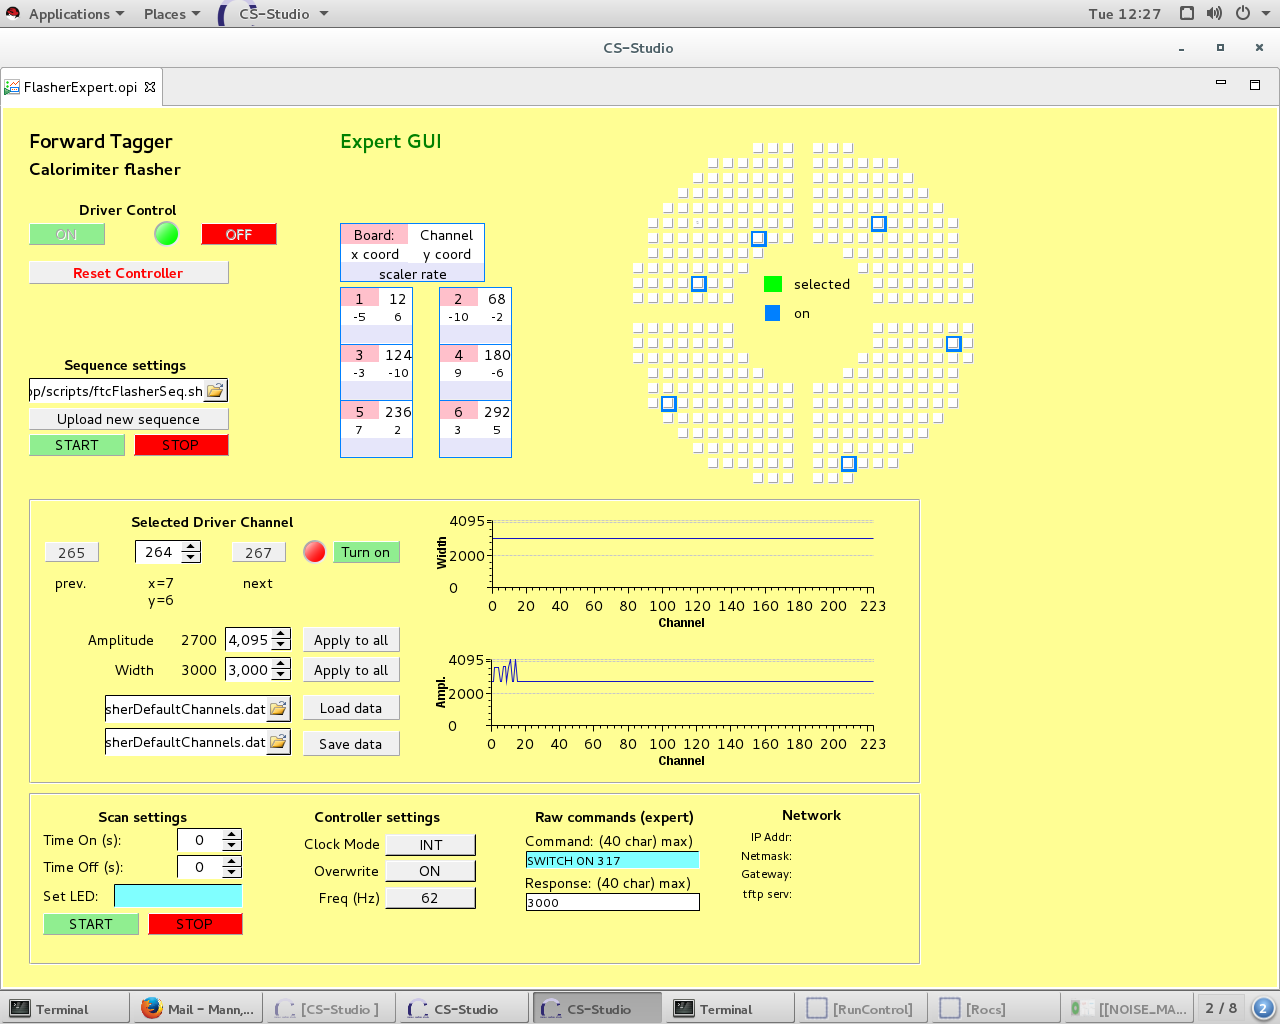
\includegraphics[width=0.85\textwidth]{pics/FTC_flasher_Expert.png}
\caption{\label{fig:LEDexpert} View of the LED flasher expert controls.}
\end{figure}
%\%\%\%\%\%\%\%\%\%\%\%\%\%\%\%\%\%\%\%\%\%\%\%\%\%\%\%\

\begin{enumerate}
\item{\textbf{Getting There!}}
\begin{itemize}
\item Using the Hall-B Epics main window select the option FTC Flasher Expert.\ref{fig:EPICSmain}  Within this GUi the user has master control of all the LED Flasher's capabilities. The User may flash groups or single LED's automatically, set LED amplitudes and widths, send raw commands to the flasher, and control various trigger aspects of the flasher.
\end{itemize}

\item{\textbf{Novice: Turning on/off}}
\begin{itemize}
\item On the Flasher Gui there are two options under driver control ``ON'' and ``OFF''. Before starting anything with the LED system make sure the driver control is on, otherwise all commands you send to the GUi will have no effect. Once finished with your work, remember to switch off the system; if this action is not performed you could unwantingly trigger the system (versus a acalibration run), or flash the APD within the FTCal with an LED while taking an actual run. \ref{fig:LEDexpertTop}
\end{itemize}

\item{\textbf{Novice: Visual Map}}
\begin{itemize}
\item As with the novice window, the user can select single LED's and mouseover each element to determine the component number and LED driver channel. The only limitation of using this map is that, like with the novice version of this Gui, the user will be unable to set Amplitudes, Widths, or turn individual LED's on. \ref{fig:LEDexpertTop}
\end{itemize}

\item{\textbf{Novice: Sequence}}
\begin{itemize}
\item As with the novice window the user can also initiatestart and stop a sequence, with the corresponding buttons on the Gui. This sequece flashes a set of 6 LED's (with exception to the first step, in which only 2 a flashed) at a time for a total of 60 seconds. The 3X2 matrix in the middle shows the current LED's being activated as well as their coordinate positions in the FTCal.  \ref{fig:LEDexpertTop}
\end{itemize}

%\%\%\%\%\%\%\%\%\%\%\%\%\%\%\%\%\%\%\%\%\%\%\%\%\%\%\%\
\begin{figure}[htbp]
\center
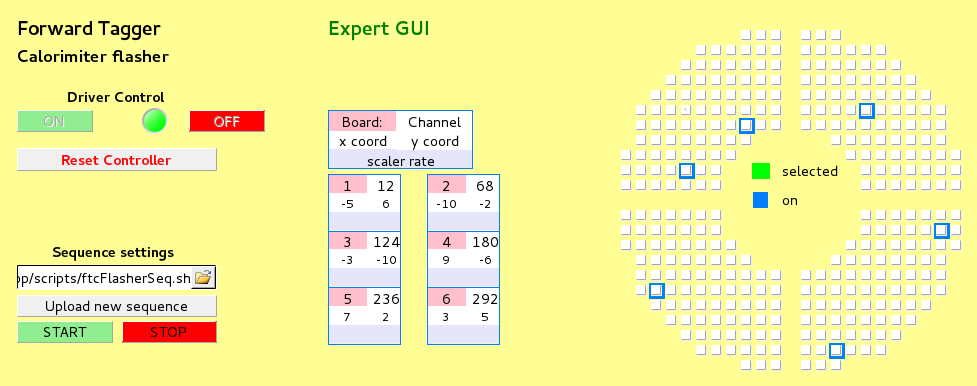
\includegraphics[width=0.85\textwidth]{pics/FTC_flasher_Expert_Top.png}
\caption{\label{fig:LEDexpertTop} Cropped view of the LED flasher expert controls, showing only the top section.}
\end{figure}
%\%\%\%\%\%\%\%\%\%\%\%\%\%\%\%\%\%\%\%\%\%\%\%\%\%\%\%\

\item{\textbf{Expert: Single Selection}}
\begin{itemize}
\item In the middle section of the GUi the user will see the options to cycle through each LED in order, starting at (3,11), and transitioning horizontally accross the row when the next LED is selected. Most importantly the user will also be given the opportunity to turn on/off individual LED's for specific channel testing. The numbering system is highlighted in the image below. \ref{fig:LEDnumb} \ref{fig:LEDexpertMid}
\end{itemize}

\item{\textbf{Expert: Amplitudes and Widths}}
\begin{itemize}
\item In the middle section of the Gui, the user will also be allowed to alter the flashing LED's amplitude (brightness), and width (the length of the pulse flash); two graphs on the right side of the window display the distribution of amplitudes and widths for all LEDs. If the user would like to save/load their own settings for all LED's the save/load buttons will perform that task. \ref{fig:LEDexpertMid}
\end{itemize}

%\%\%\%\%\%\%\%\%\%\%\%\%\%\%\%\%\%\%\%\%\%\%\%\%\%\%\%\
\begin{figure}[htbp]
\center
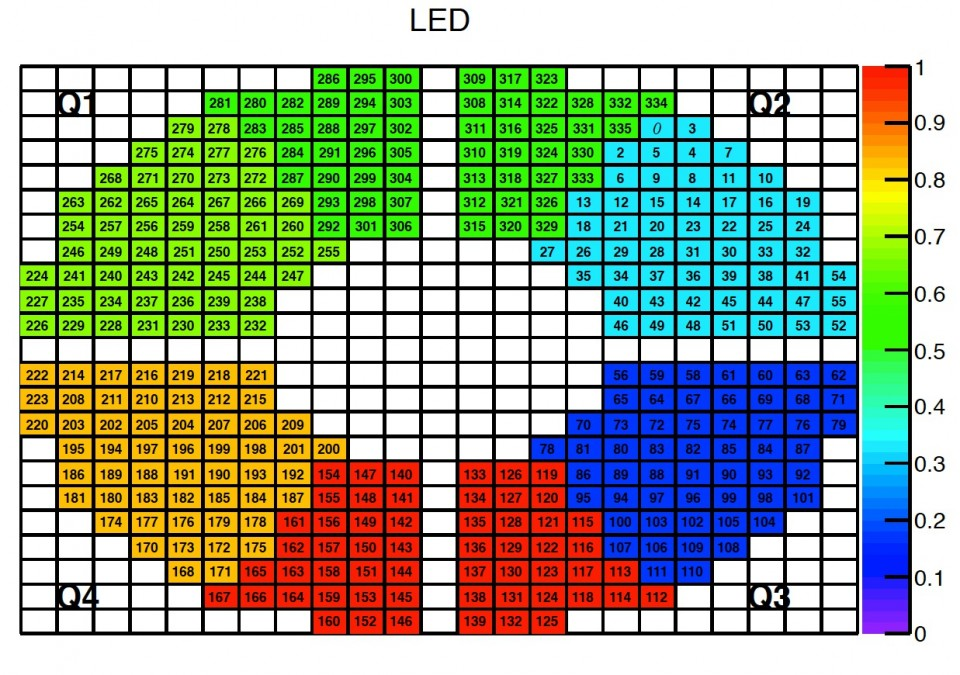
\includegraphics[width=0.85\textwidth]{pics/FT-CalMap-LED_Numb.jpg}
\caption{\label{fig:LEDnumb} LED number association.}
\end{figure}
%\%\%\%\%\%\%\%\%\%\%\%\%\%\%\%\%\%\%\%\%\%\%\%\%\%\%\%\

%\%\%\%\%\%\%\%\%\%\%\%\%\%\%\%\%\%\%\%\%\%\%\%\%\%\%\%\
\begin{figure}[htbp]
\center
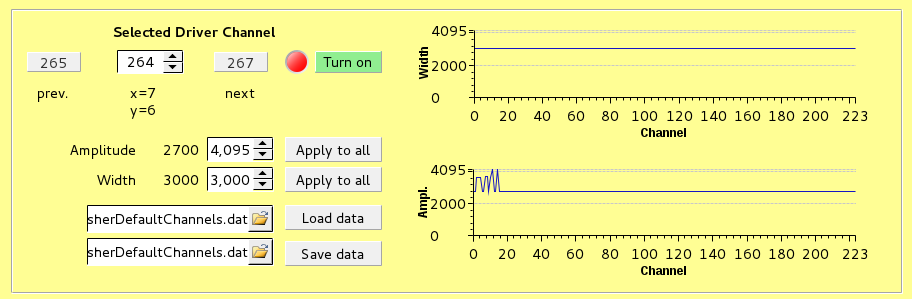
\includegraphics[width=0.85\textwidth]{pics/FTC_flasher_Expert_Mid.png}
\caption{\label{fig:LEDexpertMid} Cropped view of the LED flasher expert controls, showing only the middle section.}
\end{figure}
%\%\%\%\%\%\%\%\%\%\%\%\%\%\%\%\%\%\%\%\%\%\%\%\%\%\%\%\


\item{\textbf{Expert: Scan Setting}}
\begin{itemize}
\item ****TO BE ADDED*****
\end{itemize}

\item{\textbf{Expert: Controller Setting (Trigger)}}
\begin{itemize}
\item Under this column the three buttons displayed allow the user to trigger to the entire system, alter the rates of this trigger, and enable an overwrite function. the  two options related to the trigger are: ``Clock Mode'' and ``Freq (Hz)''.The final button ``Overwrite'' allows the user to continually turn on LEDs without having to turn off the previously selected channel. \ref{fig:LEDexpertBot}
\end{itemize}

\item{\textbf{Expert: Raw Commands}}
\begin{itemize}
\item In order to use this section the user will need to be familiar with the list of raw commands that the flasher can accept. The list of commands is found on the following WIKI page: 
https://wiki.ge.infn.it/g3wiki/index.php/Monitoring\_system\#For\_dummies in the section title ``List of available commands''  \ref{fig:LEDexpertBot}
\end{itemize}

\item{\textbf{Expert: Network Information}}
\begin{itemize}
\item  ****TO BE ADDED*****
\end{itemize}

%\%\%\%\%\%\%\%\%\%\%\%\%\%\%\%\%\%\%\%\%\%\%\%\%\%\%\%\
\begin{figure}[htbp]
\center
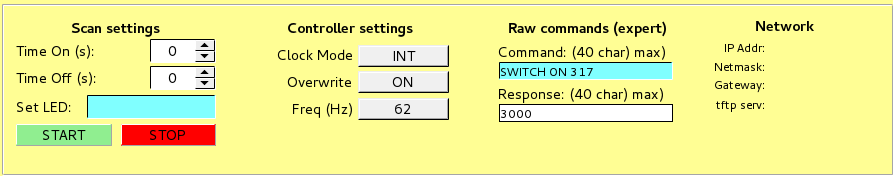
\includegraphics[width=0.85\textwidth]{pics/FTC_flasher_Expert_Bot.png}
\caption{\label{fig:LEDexpertBot} Cropped view of the LED flasher expert controls, showing only the bottom section.}
\end{figure}
%\%\%\%\%\%\%\%\%\%\%\%\%\%\%\%\%\%\%\%\%\%\%\%\%\%\%\%\

\end{enumerate}



\end{document}
